\documentclass[11pt]{article}

% Shared notes settings for Applied Machine Learning lectures (UPES).
% Keep this file free of \documentclass to allow reuse via \input.

\usepackage[utf8]{inputenc}
\usepackage[T1]{fontenc}
\usepackage{lmodern}          % scalable T1 fonts; without this pdflatex falls back
\input{glyphtounicode}        % to bitmapped EC Type 3 and the PDFs are neither
\pdfgentounicode=1            % searchable nor screen-reader friendly
\usepackage[a4paper,margin=1in]{geometry}
\usepackage{hyperref}
\usepackage{xurl}
\usepackage{booktabs}
\usepackage{amsmath}
\usepackage{amssymb}
\usepackage{listings}
\usepackage{xcolor}
\usepackage{enumitem}
\usepackage{parskip}

% Code listings (Python-oriented for this subject).
\lstset{
  language=Python,
  basicstyle=\ttfamily\small,
  keywordstyle=\color{blue},
  commentstyle=\color{gray},
  stringstyle=\color{teal},
  showstringspaces=false,
  columns=fullflexible,
  frame=single,
  framerule=0.2pt,
  breaklines=true
}

\setlist[itemize]{topsep=0.3em,itemsep=0.2em}
\setlist[enumerate]{topsep=0.3em,itemsep=0.2em}

% Simple per-section source line.
\newcommand{\notesources}[1]{\par\noindent{\small\color{gray}\textit{Sources:} \sloppy #1\par}}

% Unit-wise source strings for this subject (used by slides + notes).
% Path is relative to the lecture `latex/` folder (the compilation CWD).
\IfFileExists{../../../_shared/aml-sources.tex}{%
  % Source strings for Applied Machine Learning (CSAI2017P) — used by slides + notes.
% Prescribed texts and reference books are taken from the course syllabus.
% Support texts are the author-hosted open-access editions:
%   statlearning.com            (ISL with Python)
%   probml.github.io/pml-book   (Murphy, Probabilistic Machine Learning)
%   d2l.ai                      (Dive into Deep Learning)
%   mml-book.github.io          (Mathematics for Machine Learning)

\newcommand{\AMLRepoURL}{https://github.com/tali7c/Applied-Machine-Learning}

% --- prescribed -------------------------------------------------------------
\newcommand{\AMLPrescribed}{%
M\"uller and Guido, \textit{Introduction to Machine Learning with Python}, O'Reilly, 2016.;%
Bishop, \textit{Pattern Recognition and Machine Learning}, Springer, 2006.;%
Murphy, \textit{Machine Learning: A Probabilistic Perspective}, MIT Press, 2012.;%
Han, Kamber and Pei, \textit{Data Mining: Concepts and Techniques} (3e), Morgan Kaufmann, 2012.%
}

% --- unit-wise ---------------------------------------------------------------
\newcommand{\AMLUnitISources}{%
M\"uller and Guido, \textit{Introduction to Machine Learning with Python}, Ch. 1.;%
Bishop, \textit{Pattern Recognition and Machine Learning}, Ch. 1.;%
Murphy, \textit{Probabilistic Machine Learning: An Introduction}, MIT Press, 2022, Ch. 1.;%
Mitchell, \textit{Machine Learning}, McGraw Hill, 1997, Ch. 1.;%
Scikit-learn documentation, accessed 2026-08-04.%
}

\newcommand{\AMLUnitIISources}{%
Bishop, \textit{Pattern Recognition and Machine Learning}, \S1.5, \S4.3, \S7.1.;%
Zhang, Lipton, Li and Smola, \textit{Dive into Deep Learning}, \S3.4.;%
Shalev-Shwartz and Ben-David, \textit{Understanding Machine Learning}, Ch. 15.;%
Murphy, \textit{Probabilistic Machine Learning: An Introduction}, Ch. 5.%
}

\newcommand{\AMLUnitIIISources}{%
Zhang, Lipton, Li and Smola, \textit{Dive into Deep Learning}, Ch. 12 (Optimization Algorithms).;%
Deisenroth, Faisal and Ong, \textit{Mathematics for Machine Learning}, Ch. 7.;%
Kingma and Ba, ``Adam: A Method for Stochastic Optimization,'' ICLR 2015.;%
Ruder, ``An overview of gradient descent optimization algorithms,'' arXiv:1609.04747, 2016.%
}

\newcommand{\AMLUnitIVSources}{%
Han, Kamber and Pei, \textit{Data Mining: Concepts and Techniques} (3e), Ch. 3.;%
M\"uller and Guido, \textit{Introduction to Machine Learning with Python}, Ch. 3--4.;%
James, Witten, Hastie, Tibshirani and Taylor, \textit{An Introduction to Statistical Learning with Python}, Ch. 5--6, 12.;%
Scikit-learn documentation (preprocessing, model selection), accessed 2026-08-04.%
}

\newcommand{\AMLUnitVSources}{%
James et al., \textit{An Introduction to Statistical Learning with Python}, Ch. 3--6.;%
Bishop, \textit{Pattern Recognition and Machine Learning}, Ch. 3.;%
Deisenroth, Faisal and Ong, \textit{Mathematics for Machine Learning}, Ch. 9.;%
M\"uller and Guido, \textit{Introduction to Machine Learning with Python}, \S2.3.%
}

\newcommand{\AMLUnitVISources}{%
Han, Kamber and Pei, \textit{Data Mining: Concepts and Techniques} (3e), Ch. 8--9.;%
James et al., \textit{An Introduction to Statistical Learning with Python}, Ch. 8--9.;%
Bishop, \textit{Pattern Recognition and Machine Learning}, Ch. 4--5, 7, 14.;%
Zhang et al., \textit{Dive into Deep Learning}, Ch. 5.%
}

\newcommand{\AMLUnitVIISources}{%
Han, Kamber and Pei, \textit{Data Mining: Concepts and Techniques} (3e), Ch. 10.;%
James et al., \textit{An Introduction to Statistical Learning with Python}, Ch. 12.;%
M\"uller and Guido, \textit{Introduction to Machine Learning with Python}, \S3.5.;%
Ester, Kriegel, Sander and Xu, ``A density-based algorithm for discovering clusters (DBSCAN),'' KDD 1996.%
}

\newcommand{\AMLLabSources}{%
M\"uller and Guido, \textit{Introduction to Machine Learning with Python}, companion notebooks.;%
McKinney, \textit{Python for Data Analysis} (3e), O'Reilly, 2022.;%
Scikit-learn user guide, accessed 2026-08-04.;%
Matplotlib and Seaborn documentation, accessed 2026-08-04.%
}
%
}{%
  % Faculty copies live under `private/` so their compile CWD is different.
  \IfFileExists{../../../../public/_shared/aml-sources.tex}{%
    % Source strings for Applied Machine Learning (CSAI2017P) — used by slides + notes.
% Prescribed texts and reference books are taken from the course syllabus.
% Support texts are the author-hosted open-access editions:
%   statlearning.com            (ISL with Python)
%   probml.github.io/pml-book   (Murphy, Probabilistic Machine Learning)
%   d2l.ai                      (Dive into Deep Learning)
%   mml-book.github.io          (Mathematics for Machine Learning)

\newcommand{\AMLRepoURL}{https://github.com/tali7c/Applied-Machine-Learning}

% --- prescribed -------------------------------------------------------------
\newcommand{\AMLPrescribed}{%
M\"uller and Guido, \textit{Introduction to Machine Learning with Python}, O'Reilly, 2016.;%
Bishop, \textit{Pattern Recognition and Machine Learning}, Springer, 2006.;%
Murphy, \textit{Machine Learning: A Probabilistic Perspective}, MIT Press, 2012.;%
Han, Kamber and Pei, \textit{Data Mining: Concepts and Techniques} (3e), Morgan Kaufmann, 2012.%
}

% --- unit-wise ---------------------------------------------------------------
\newcommand{\AMLUnitISources}{%
M\"uller and Guido, \textit{Introduction to Machine Learning with Python}, Ch. 1.;%
Bishop, \textit{Pattern Recognition and Machine Learning}, Ch. 1.;%
Murphy, \textit{Probabilistic Machine Learning: An Introduction}, MIT Press, 2022, Ch. 1.;%
Mitchell, \textit{Machine Learning}, McGraw Hill, 1997, Ch. 1.;%
Scikit-learn documentation, accessed 2026-08-04.%
}

\newcommand{\AMLUnitIISources}{%
Bishop, \textit{Pattern Recognition and Machine Learning}, \S1.5, \S4.3, \S7.1.;%
Zhang, Lipton, Li and Smola, \textit{Dive into Deep Learning}, \S3.4.;%
Shalev-Shwartz and Ben-David, \textit{Understanding Machine Learning}, Ch. 15.;%
Murphy, \textit{Probabilistic Machine Learning: An Introduction}, Ch. 5.%
}

\newcommand{\AMLUnitIIISources}{%
Zhang, Lipton, Li and Smola, \textit{Dive into Deep Learning}, Ch. 12 (Optimization Algorithms).;%
Deisenroth, Faisal and Ong, \textit{Mathematics for Machine Learning}, Ch. 7.;%
Kingma and Ba, ``Adam: A Method for Stochastic Optimization,'' ICLR 2015.;%
Ruder, ``An overview of gradient descent optimization algorithms,'' arXiv:1609.04747, 2016.%
}

\newcommand{\AMLUnitIVSources}{%
Han, Kamber and Pei, \textit{Data Mining: Concepts and Techniques} (3e), Ch. 3.;%
M\"uller and Guido, \textit{Introduction to Machine Learning with Python}, Ch. 3--4.;%
James, Witten, Hastie, Tibshirani and Taylor, \textit{An Introduction to Statistical Learning with Python}, Ch. 5--6, 12.;%
Scikit-learn documentation (preprocessing, model selection), accessed 2026-08-04.%
}

\newcommand{\AMLUnitVSources}{%
James et al., \textit{An Introduction to Statistical Learning with Python}, Ch. 3--6.;%
Bishop, \textit{Pattern Recognition and Machine Learning}, Ch. 3.;%
Deisenroth, Faisal and Ong, \textit{Mathematics for Machine Learning}, Ch. 9.;%
M\"uller and Guido, \textit{Introduction to Machine Learning with Python}, \S2.3.%
}

\newcommand{\AMLUnitVISources}{%
Han, Kamber and Pei, \textit{Data Mining: Concepts and Techniques} (3e), Ch. 8--9.;%
James et al., \textit{An Introduction to Statistical Learning with Python}, Ch. 8--9.;%
Bishop, \textit{Pattern Recognition and Machine Learning}, Ch. 4--5, 7, 14.;%
Zhang et al., \textit{Dive into Deep Learning}, Ch. 5.%
}

\newcommand{\AMLUnitVIISources}{%
Han, Kamber and Pei, \textit{Data Mining: Concepts and Techniques} (3e), Ch. 10.;%
James et al., \textit{An Introduction to Statistical Learning with Python}, Ch. 12.;%
M\"uller and Guido, \textit{Introduction to Machine Learning with Python}, \S3.5.;%
Ester, Kriegel, Sander and Xu, ``A density-based algorithm for discovering clusters (DBSCAN),'' KDD 1996.%
}

\newcommand{\AMLLabSources}{%
M\"uller and Guido, \textit{Introduction to Machine Learning with Python}, companion notebooks.;%
McKinney, \textit{Python for Data Analysis} (3e), O'Reilly, 2022.;%
Scikit-learn user guide, accessed 2026-08-04.;%
Matplotlib and Seaborn documentation, accessed 2026-08-04.%
}
%
  }{%
    % Question papers live at `private/<family>/<instrument>/`.
    \IfFileExists{../../../public/_shared/aml-sources.tex}{%
      % Source strings for Applied Machine Learning (CSAI2017P) — used by slides + notes.
% Prescribed texts and reference books are taken from the course syllabus.
% Support texts are the author-hosted open-access editions:
%   statlearning.com            (ISL with Python)
%   probml.github.io/pml-book   (Murphy, Probabilistic Machine Learning)
%   d2l.ai                      (Dive into Deep Learning)
%   mml-book.github.io          (Mathematics for Machine Learning)

\newcommand{\AMLRepoURL}{https://github.com/tali7c/Applied-Machine-Learning}

% --- prescribed -------------------------------------------------------------
\newcommand{\AMLPrescribed}{%
M\"uller and Guido, \textit{Introduction to Machine Learning with Python}, O'Reilly, 2016.;%
Bishop, \textit{Pattern Recognition and Machine Learning}, Springer, 2006.;%
Murphy, \textit{Machine Learning: A Probabilistic Perspective}, MIT Press, 2012.;%
Han, Kamber and Pei, \textit{Data Mining: Concepts and Techniques} (3e), Morgan Kaufmann, 2012.%
}

% --- unit-wise ---------------------------------------------------------------
\newcommand{\AMLUnitISources}{%
M\"uller and Guido, \textit{Introduction to Machine Learning with Python}, Ch. 1.;%
Bishop, \textit{Pattern Recognition and Machine Learning}, Ch. 1.;%
Murphy, \textit{Probabilistic Machine Learning: An Introduction}, MIT Press, 2022, Ch. 1.;%
Mitchell, \textit{Machine Learning}, McGraw Hill, 1997, Ch. 1.;%
Scikit-learn documentation, accessed 2026-08-04.%
}

\newcommand{\AMLUnitIISources}{%
Bishop, \textit{Pattern Recognition and Machine Learning}, \S1.5, \S4.3, \S7.1.;%
Zhang, Lipton, Li and Smola, \textit{Dive into Deep Learning}, \S3.4.;%
Shalev-Shwartz and Ben-David, \textit{Understanding Machine Learning}, Ch. 15.;%
Murphy, \textit{Probabilistic Machine Learning: An Introduction}, Ch. 5.%
}

\newcommand{\AMLUnitIIISources}{%
Zhang, Lipton, Li and Smola, \textit{Dive into Deep Learning}, Ch. 12 (Optimization Algorithms).;%
Deisenroth, Faisal and Ong, \textit{Mathematics for Machine Learning}, Ch. 7.;%
Kingma and Ba, ``Adam: A Method for Stochastic Optimization,'' ICLR 2015.;%
Ruder, ``An overview of gradient descent optimization algorithms,'' arXiv:1609.04747, 2016.%
}

\newcommand{\AMLUnitIVSources}{%
Han, Kamber and Pei, \textit{Data Mining: Concepts and Techniques} (3e), Ch. 3.;%
M\"uller and Guido, \textit{Introduction to Machine Learning with Python}, Ch. 3--4.;%
James, Witten, Hastie, Tibshirani and Taylor, \textit{An Introduction to Statistical Learning with Python}, Ch. 5--6, 12.;%
Scikit-learn documentation (preprocessing, model selection), accessed 2026-08-04.%
}

\newcommand{\AMLUnitVSources}{%
James et al., \textit{An Introduction to Statistical Learning with Python}, Ch. 3--6.;%
Bishop, \textit{Pattern Recognition and Machine Learning}, Ch. 3.;%
Deisenroth, Faisal and Ong, \textit{Mathematics for Machine Learning}, Ch. 9.;%
M\"uller and Guido, \textit{Introduction to Machine Learning with Python}, \S2.3.%
}

\newcommand{\AMLUnitVISources}{%
Han, Kamber and Pei, \textit{Data Mining: Concepts and Techniques} (3e), Ch. 8--9.;%
James et al., \textit{An Introduction to Statistical Learning with Python}, Ch. 8--9.;%
Bishop, \textit{Pattern Recognition and Machine Learning}, Ch. 4--5, 7, 14.;%
Zhang et al., \textit{Dive into Deep Learning}, Ch. 5.%
}

\newcommand{\AMLUnitVIISources}{%
Han, Kamber and Pei, \textit{Data Mining: Concepts and Techniques} (3e), Ch. 10.;%
James et al., \textit{An Introduction to Statistical Learning with Python}, Ch. 12.;%
M\"uller and Guido, \textit{Introduction to Machine Learning with Python}, \S3.5.;%
Ester, Kriegel, Sander and Xu, ``A density-based algorithm for discovering clusters (DBSCAN),'' KDD 1996.%
}

\newcommand{\AMLLabSources}{%
M\"uller and Guido, \textit{Introduction to Machine Learning with Python}, companion notebooks.;%
McKinney, \textit{Python for Data Analysis} (3e), O'Reilly, 2022.;%
Scikit-learn user guide, accessed 2026-08-04.;%
Matplotlib and Seaborn documentation, accessed 2026-08-04.%
}
%
    }{%
      % Marking schemes live at `private/solutions/<family>/<id>/latex/`.
      \IfFileExists{../../../../../public/_shared/aml-sources.tex}{%
        % Source strings for Applied Machine Learning (CSAI2017P) — used by slides + notes.
% Prescribed texts and reference books are taken from the course syllabus.
% Support texts are the author-hosted open-access editions:
%   statlearning.com            (ISL with Python)
%   probml.github.io/pml-book   (Murphy, Probabilistic Machine Learning)
%   d2l.ai                      (Dive into Deep Learning)
%   mml-book.github.io          (Mathematics for Machine Learning)

\newcommand{\AMLRepoURL}{https://github.com/tali7c/Applied-Machine-Learning}

% --- prescribed -------------------------------------------------------------
\newcommand{\AMLPrescribed}{%
M\"uller and Guido, \textit{Introduction to Machine Learning with Python}, O'Reilly, 2016.;%
Bishop, \textit{Pattern Recognition and Machine Learning}, Springer, 2006.;%
Murphy, \textit{Machine Learning: A Probabilistic Perspective}, MIT Press, 2012.;%
Han, Kamber and Pei, \textit{Data Mining: Concepts and Techniques} (3e), Morgan Kaufmann, 2012.%
}

% --- unit-wise ---------------------------------------------------------------
\newcommand{\AMLUnitISources}{%
M\"uller and Guido, \textit{Introduction to Machine Learning with Python}, Ch. 1.;%
Bishop, \textit{Pattern Recognition and Machine Learning}, Ch. 1.;%
Murphy, \textit{Probabilistic Machine Learning: An Introduction}, MIT Press, 2022, Ch. 1.;%
Mitchell, \textit{Machine Learning}, McGraw Hill, 1997, Ch. 1.;%
Scikit-learn documentation, accessed 2026-08-04.%
}

\newcommand{\AMLUnitIISources}{%
Bishop, \textit{Pattern Recognition and Machine Learning}, \S1.5, \S4.3, \S7.1.;%
Zhang, Lipton, Li and Smola, \textit{Dive into Deep Learning}, \S3.4.;%
Shalev-Shwartz and Ben-David, \textit{Understanding Machine Learning}, Ch. 15.;%
Murphy, \textit{Probabilistic Machine Learning: An Introduction}, Ch. 5.%
}

\newcommand{\AMLUnitIIISources}{%
Zhang, Lipton, Li and Smola, \textit{Dive into Deep Learning}, Ch. 12 (Optimization Algorithms).;%
Deisenroth, Faisal and Ong, \textit{Mathematics for Machine Learning}, Ch. 7.;%
Kingma and Ba, ``Adam: A Method for Stochastic Optimization,'' ICLR 2015.;%
Ruder, ``An overview of gradient descent optimization algorithms,'' arXiv:1609.04747, 2016.%
}

\newcommand{\AMLUnitIVSources}{%
Han, Kamber and Pei, \textit{Data Mining: Concepts and Techniques} (3e), Ch. 3.;%
M\"uller and Guido, \textit{Introduction to Machine Learning with Python}, Ch. 3--4.;%
James, Witten, Hastie, Tibshirani and Taylor, \textit{An Introduction to Statistical Learning with Python}, Ch. 5--6, 12.;%
Scikit-learn documentation (preprocessing, model selection), accessed 2026-08-04.%
}

\newcommand{\AMLUnitVSources}{%
James et al., \textit{An Introduction to Statistical Learning with Python}, Ch. 3--6.;%
Bishop, \textit{Pattern Recognition and Machine Learning}, Ch. 3.;%
Deisenroth, Faisal and Ong, \textit{Mathematics for Machine Learning}, Ch. 9.;%
M\"uller and Guido, \textit{Introduction to Machine Learning with Python}, \S2.3.%
}

\newcommand{\AMLUnitVISources}{%
Han, Kamber and Pei, \textit{Data Mining: Concepts and Techniques} (3e), Ch. 8--9.;%
James et al., \textit{An Introduction to Statistical Learning with Python}, Ch. 8--9.;%
Bishop, \textit{Pattern Recognition and Machine Learning}, Ch. 4--5, 7, 14.;%
Zhang et al., \textit{Dive into Deep Learning}, Ch. 5.%
}

\newcommand{\AMLUnitVIISources}{%
Han, Kamber and Pei, \textit{Data Mining: Concepts and Techniques} (3e), Ch. 10.;%
James et al., \textit{An Introduction to Statistical Learning with Python}, Ch. 12.;%
M\"uller and Guido, \textit{Introduction to Machine Learning with Python}, \S3.5.;%
Ester, Kriegel, Sander and Xu, ``A density-based algorithm for discovering clusters (DBSCAN),'' KDD 1996.%
}

\newcommand{\AMLLabSources}{%
M\"uller and Guido, \textit{Introduction to Machine Learning with Python}, companion notebooks.;%
McKinney, \textit{Python for Data Analysis} (3e), O'Reilly, 2022.;%
Scikit-learn user guide, accessed 2026-08-04.;%
Matplotlib and Seaborn documentation, accessed 2026-08-04.%
}
%
      }{%
        % Source strings for Applied Machine Learning (CSAI2017P) — used by slides + notes.
% Prescribed texts and reference books are taken from the course syllabus.
% Support texts are the author-hosted open-access editions:
%   statlearning.com            (ISL with Python)
%   probml.github.io/pml-book   (Murphy, Probabilistic Machine Learning)
%   d2l.ai                      (Dive into Deep Learning)
%   mml-book.github.io          (Mathematics for Machine Learning)

\newcommand{\AMLRepoURL}{https://github.com/tali7c/Applied-Machine-Learning}

% --- prescribed -------------------------------------------------------------
\newcommand{\AMLPrescribed}{%
M\"uller and Guido, \textit{Introduction to Machine Learning with Python}, O'Reilly, 2016.;%
Bishop, \textit{Pattern Recognition and Machine Learning}, Springer, 2006.;%
Murphy, \textit{Machine Learning: A Probabilistic Perspective}, MIT Press, 2012.;%
Han, Kamber and Pei, \textit{Data Mining: Concepts and Techniques} (3e), Morgan Kaufmann, 2012.%
}

% --- unit-wise ---------------------------------------------------------------
\newcommand{\AMLUnitISources}{%
M\"uller and Guido, \textit{Introduction to Machine Learning with Python}, Ch. 1.;%
Bishop, \textit{Pattern Recognition and Machine Learning}, Ch. 1.;%
Murphy, \textit{Probabilistic Machine Learning: An Introduction}, MIT Press, 2022, Ch. 1.;%
Mitchell, \textit{Machine Learning}, McGraw Hill, 1997, Ch. 1.;%
Scikit-learn documentation, accessed 2026-08-04.%
}

\newcommand{\AMLUnitIISources}{%
Bishop, \textit{Pattern Recognition and Machine Learning}, \S1.5, \S4.3, \S7.1.;%
Zhang, Lipton, Li and Smola, \textit{Dive into Deep Learning}, \S3.4.;%
Shalev-Shwartz and Ben-David, \textit{Understanding Machine Learning}, Ch. 15.;%
Murphy, \textit{Probabilistic Machine Learning: An Introduction}, Ch. 5.%
}

\newcommand{\AMLUnitIIISources}{%
Zhang, Lipton, Li and Smola, \textit{Dive into Deep Learning}, Ch. 12 (Optimization Algorithms).;%
Deisenroth, Faisal and Ong, \textit{Mathematics for Machine Learning}, Ch. 7.;%
Kingma and Ba, ``Adam: A Method for Stochastic Optimization,'' ICLR 2015.;%
Ruder, ``An overview of gradient descent optimization algorithms,'' arXiv:1609.04747, 2016.%
}

\newcommand{\AMLUnitIVSources}{%
Han, Kamber and Pei, \textit{Data Mining: Concepts and Techniques} (3e), Ch. 3.;%
M\"uller and Guido, \textit{Introduction to Machine Learning with Python}, Ch. 3--4.;%
James, Witten, Hastie, Tibshirani and Taylor, \textit{An Introduction to Statistical Learning with Python}, Ch. 5--6, 12.;%
Scikit-learn documentation (preprocessing, model selection), accessed 2026-08-04.%
}

\newcommand{\AMLUnitVSources}{%
James et al., \textit{An Introduction to Statistical Learning with Python}, Ch. 3--6.;%
Bishop, \textit{Pattern Recognition and Machine Learning}, Ch. 3.;%
Deisenroth, Faisal and Ong, \textit{Mathematics for Machine Learning}, Ch. 9.;%
M\"uller and Guido, \textit{Introduction to Machine Learning with Python}, \S2.3.%
}

\newcommand{\AMLUnitVISources}{%
Han, Kamber and Pei, \textit{Data Mining: Concepts and Techniques} (3e), Ch. 8--9.;%
James et al., \textit{An Introduction to Statistical Learning with Python}, Ch. 8--9.;%
Bishop, \textit{Pattern Recognition and Machine Learning}, Ch. 4--5, 7, 14.;%
Zhang et al., \textit{Dive into Deep Learning}, Ch. 5.%
}

\newcommand{\AMLUnitVIISources}{%
Han, Kamber and Pei, \textit{Data Mining: Concepts and Techniques} (3e), Ch. 10.;%
James et al., \textit{An Introduction to Statistical Learning with Python}, Ch. 12.;%
M\"uller and Guido, \textit{Introduction to Machine Learning with Python}, \S3.5.;%
Ester, Kriegel, Sander and Xu, ``A density-based algorithm for discovering clusters (DBSCAN),'' KDD 1996.%
}

\newcommand{\AMLLabSources}{%
M\"uller and Guido, \textit{Introduction to Machine Learning with Python}, companion notebooks.;%
McKinney, \textit{Python for Data Analysis} (3e), O'Reilly, 2022.;%
Scikit-learn user guide, accessed 2026-08-04.;%
Matplotlib and Seaborn documentation, accessed 2026-08-04.%
}
%
      }%
    }%
  }%
}


\graphicspath{{../figures/}}

% Local to this document: better line breaking in a text-dense set of notes.
\usepackage{microtype}
% Text-dense notes: slightly tighter paragraph separation than the shared default.
\setlength{\parskip}{0.40\baselineskip plus 2pt}

% This lecture pairs almost every paragraph with a listing and its output, so
% the default \medskipamount around each block adds up to several pages.
\lstset{aboveskip=2pt, belowskip=2pt}
\lstdefinestyle{amlout}{language={}, keepspaces=true,
  basicstyle=\ttfamily\footnotesize\color{black!80},
  backgroundcolor=\color{black!4}, frame=leftline, framerule=2pt,
  rulecolor=\color{black!25}, breaklines=true, columns=fullflexible,
  xleftmargin=8pt, aboveskip=1pt, belowskip=3pt, literate={-}{{-}}1}
\captionsetup{skip=4pt, font=small}
% Fifteen wide figures in a text-dense document: let them share pages with
% prose instead of being pushed onto float pages of their own.
\renewcommand{\topfraction}{0.92}
\renewcommand{\bottomfraction}{0.75}
\renewcommand{\textfraction}{0.06}
\renewcommand{\floatpagefraction}{0.85}
\setlength{\floatsep}{4pt plus 2pt minus 2pt}
\setlength{\textfloatsep}{6pt plus 2pt minus 2pt}
\setlength{\intextsep}{6pt plus 2pt minus 2pt}

\title{Applied Machine Learning\\Unit 05 --- Lecture 09 Notes\\
       Maximum Likelihood, Model Adequacy and Over-fitting}
\author{Tofik Ali}
\date{Autumn 2026}

\begin{document}
\maketitle

\begin{keyidea}[Read this first]
These notes are written so that you can learn the material \emph{without}
having been in the lecture. Every concept is developed from scratch, every
number you see was produced by running the code shown beside it, and every
figure was generated from real computation rather than drawn by hand.

The previous lecture produced an estimator. It set up simple linear
regression, minimised the sum of squared errors, and arrived at the closed
form $b_1 = S_{xy}/S_{xx}$, $b_0 = \bar y - b_1\bar x$. It did not say
\emph{why} the sum of squares.

This lecture answers that, and the answer is the central result here:
\textbf{write down a Gaussian probability model for the noise, form the
likelihood, take logarithms, and maximising the likelihood turns out to be
identical to minimising the sum of squared errors.} Least squares is not a
convenient guess. It is the maximum likelihood estimate under a specific,
checkable assumption --- and once you know which assumption, you know what to
check.

The rest of the lecture is that checking. $R^2$ in three lines of arithmetic,
and then two facts about it that decide whether you can trust a reported
number: it \textbf{never decreases} when you add a predictor, even a column of
pure noise, and on held-out data it can be \textbf{negative without limit}.
Then residual plots, which see everything $R^2$ cannot. Then over-fitting ---
where training error falls at every step while test error turns up --- and
cross-validation, which detects the turn without ever opening the test set.

The single result to carry out of the lecture: on $30$ rows,
\textbf{$27$ columns of pure noise raised $R^2$ from $0.2413$ to $0.9401$ and
it never decreased once}. Work through Section~\ref{sec:noisecols} with a
Python session open until you can say exactly why that had to happen.
\end{keyidea}

{\small\tableofcontents}
\medskip

% =========================================================================
\section{How to use these notes}
\label{sec:how}

Read in order. Section~\ref{sec:mle} is the mathematical core and everything
after it depends on it; Section~\ref{sec:r2} assumes the normal equations of
Lecture~8; Section~\ref{sec:cv} is the payoff for
Section~\ref{sec:overfit}. The mathematics used is one product, one logarithm,
two partial derivatives and one expectation. If you can differentiate
$\log \sigma^2$ you have everything you need.

There are four kinds of box. \textbf{Key idea} --- the one sentence to
remember a month from now. \textbf{Worked example} --- a calculation done by
hand, with small numbers, before any library is used. \textbf{Caution} --- the
specific mistake that section exists to prevent. \textbf{Try it yourself} ---
something to run, with the expected output given so you can check.

Code appears in a framed block, and directly beneath it a shaded block showing
what that code \emph{actually printed}. If you run it and get something
different, trust your machine and tell me.

One set of five points runs through the whole document:
\[
  x = (1,2,3,4,5), \qquad y = (2,4,5,4,5).
\]
It appears in Section~\ref{sec:direct} for the three regression methods, in
Section~\ref{sec:mle} for the likelihood, and in Section~\ref{sec:r2hand} for
$R^2$. The numbers were chosen so that every intermediate quantity is exact:
$\bar x = 3$, $\bar y = 4$, $S_{xx} = 10$, $S_{yy} = 6$, $S_{xy} = 6$,
$b_1 = 0.6$, $b_0 = 2.2$, $\mathrm{SSE} = 2.4$, $R^2 = 0.6$.

\subsection{What you need}

\begin{lstlisting}
pip install numpy scipy scikit-learn matplotlib
\end{lstlisting}

Every number in these notes was produced with:

\begin{lstlisting}
import numpy, scipy, sklearn, matplotlib
print("numpy", numpy.__version__, "| scipy", scipy.__version__,
      "| sklearn", sklearn.__version__,
      "| matplotlib", matplotlib.__version__)
\end{lstlisting}
\begin{codeout}
numpy 2.2.6 | scipy 1.15.3 | sklearn 1.7.2 | matplotlib 3.10.9
\end{codeout}

The only real dataset used is \texttt{load\_diabetes}, which is bundled with
scikit-learn and \textbf{downloads nothing}. Everything else is either
Anscombe's published quartet, typed out in full below, or a fixed-seed
synthetic problem.

\begin{lstlisting}
from sklearn.datasets import load_diabetes
dia = load_diabetes()
Xd, yd = dia.data, dia.target.astype(float)
print(Xd.shape)
\end{lstlisting}
\begin{codeout}
load_diabetes: 442 rows, 10 real features
\end{codeout}

\begin{caution}[Do not reach for \texttt{fetch\_*}]
Every \texttt{fetch\_*} loader downloads over HTTPS, and on the campus network
those downloads fail with a certificate error you cannot fix from your machine.
Nothing in this course depends on one: use the bundled loaders
(\texttt{load\_diabetes}, \texttt{load\_breast\_cancer}, \texttt{load\_iris},
\texttt{load\_wine}, \texttt{load\_digits}) or a fixed-seed synthetic set.
\end{caution}

\begin{keyidea}[Three kinds of seed --- the convention for this lecture]
This lecture runs more simulations than any so far, so it is worth being
explicit about where the randomness lives. There are \textbf{three} kinds of
seed here and they do different jobs.

\begin{enumerate}[leftmargin=*]
  \item \textbf{The lecture seed, $0$.} Every arbitrary draw --- the
    $20\,000$ replications of the bias simulation, the Laplace noise, the
    pure-noise columns, the heteroscedastic data, the Q--Q samples, the
    shuffled folds --- is made from \texttt{np.random.default\_rng(0)} or with
    \texttt{random\_state=0}. Nothing is special about $0$; what matters is
    that there is only one of them and that every listing shows it.
  \item \textbf{The data seed, $3$.} The $25$ points from
    $y = \sin 2\pi x + \varepsilon$ that the whole over-fitting half of the
    lecture is about are fixed by \texttt{np.random.default\_rng(3)}. That
    seed does not choose an outcome, it \emph{chooses the dataset} --- so it is
    named separately and left alone, and every section that refers to ``the
    same $25$ points'' really is using the same $25$ points.
  \item \textbf{The split sweep, $0$ to $9$.} In
    Section~\ref{sec:lottery} ten different validation splits are run
    deliberately, because \emph{the disagreement between them is the result}.
    Collapsing those to one seed would delete the demonstration.
\end{enumerate}

Every number in these notes reproduces \emph{exactly} if you run the code as
written. If you get something different, the difference is in your code or
your library versions, not in chance.
\end{keyidea}

\subsection{Learning outcomes}

By the end of this lecture you should be able to:

\begin{enumerate}[leftmargin=*]
  \item State what the \textbf{direct regression method} minimises, contrast
    it with inverse and orthogonal regression, and compute all three slopes on
    a small dataset by hand (CO2).
  \item \textbf{Derive} the maximum likelihood estimator for simple linear
    regression under Gaussian noise from a blank page: state the model, write
    the likelihood, take logarithms, and show that maximising it is identical
    to minimising the sum of squared errors (CO2, CO3).
  \item Derive $\hat\sigma^2_{\mathrm{ML}} = \mathrm{SSE}/n$, explain why it is
    biased downwards by the factor $(n-2)/n$, and give the unbiased
    alternative (CO3).
  \item Compute $R^2$ by hand from $\mathrm{SS_{tot}}$ and
    $\mathrm{SS_{res}}$, verify it against $r^2$ and $b_1^2S_{xx}$, and state
    the two properties that make a reported $R^2$ untrustworthy: monotonicity
    in the number of predictors, and unboundedness below on held-out data
    (CO3).
  \item Check the adequacy of a fitted model from its residuals --- linearity,
    constant variance, normality, independence and leverage --- and say for
    each violation what it does and does not invalidate (CO3).
  \item Recognise over-fitting from the divergence of training and held-out
    error curves, state the degree at which the turn occurs for a given
    problem, and explain why the turn depends on $n$ as well as on the model
    (CO2, CO3).
  \item Use $k$-fold and leave-one-out cross-validation to detect over-fitting
    and select a model without opening the test set, and explain why a single
    validation split is not enough (CO2).
\end{enumerate}

% =========================================================================
\section{The direct regression method}
\label{sec:direct}

\subsection{``Closest'' is a choice}

Lecture~8 fitted a line by minimising $\sum_i (y_i - b_0 - b_1 x_i)^2$. That
quantity is the sum of squared \emph{vertical} distances from the points to
the line, and choosing it is a decision, not a fact about the data. Three
classical choices exist, and the regression literature names them.

\begin{itemize}[leftmargin=*]
  \item \textbf{Direct regression} (also \emph{ordinary least squares}, or
    \emph{the regression of $y$ on $x$}) minimises the sum of squared
    \textbf{vertical} distances. It treats $x$ as known exactly and places all
    the error in $y$. Slope $b_1 = S_{xy}/S_{xx}$.
  \item \textbf{Inverse regression} minimises the sum of squared
    \textbf{horizontal} distances, i.e.\ it regresses $x$ on $y$ and then
    re-expresses the fitted relation as $y$ against $x$. Slope, so expressed,
    $S_{yy}/S_{xy}$.
  \item \textbf{Orthogonal regression} (also \emph{total least squares} or
    \emph{major-axis regression}) minimises the sum of squared
    \textbf{perpendicular} distances. Its slope comes from the leading
    eigenvector of the sample covariance matrix, so it is symmetric in the two
    variables.
\end{itemize}

\begin{keyidea}
The direct method is what this course, and every examination question in it,
means by ``regression''. It is the right choice when $x$ is measured without
error and the task is to \emph{predict} $y$ from $x$. That asymmetry is a
modelling assumption, and Section~\ref{sec:mle} turns it into a probability
statement.
\end{keyidea}

\subsection{Worked: five points, three answers}
\label{sec:fivepoints}

\begin{worked}[Three defensible lines through the same five points]
Take $x = (1,2,3,4,5)$ and $y = (2,4,5,4,5)$. Then $\bar x = 3$, $\bar y = 4$,
and
\[
  S_{xx} = 4+1+0+1+4 = 10, \qquad
  S_{yy} = 4+0+1+0+1 = 6,  \qquad
  S_{xy} = 4+0+0+0+2 = 6 .
\]
\textbf{Direct.} $b_1 = S_{xy}/S_{xx} = 6/10 = 0.6$, and
$b_0 = 4 - 0.6 \times 3 = 2.2$.

\textbf{Inverse.} Regressing $x$ on $y$ gives slope $S_{xy}/S_{yy} = 6/6 = 1$;
inverting, the line expressed as $y$ against $x$ has slope
$S_{yy}/S_{xy} = 1.0$ and intercept $4 - 1 \times 3 = 1.0$.

\textbf{Orthogonal.} The sample covariance matrix (with $n-1 = 4$) is
\[
  S = \frac{1}{4}\begin{pmatrix} 10 & 6\\ 6 & 6 \end{pmatrix}
    = \begin{pmatrix} 2.5 & 1.5\\ 1.5 & 1.5 \end{pmatrix},
  \qquad
  \lambda = \frac{4 \pm \sqrt{16 - 6}}{2}
          = 3.5811,\ 0.4189 .
\]
The leading eigenvector satisfies $(2.5 - 3.5811)v_1 + 1.5 v_2 = 0$, so
$v_2/v_1 = 0.7208$, which is the slope.

All three lines pass through $(\bar x, \bar y) = (3,4)$ --- that is forced by
the intercept equation, whichever criterion you used --- and they differ only
in how they pivot about it.
\end{worked}

\begin{lstlisting}
S = np.cov(np.vstack([x, y]))              # 2x2 sample covariance, ddof=1
lam, V = np.linalg.eigh(S)
v = V[:, np.argmax(lam)]
print(Sxy / Sxx, Syy / Sxy, v[1] / v[0])
\end{lstlisting}
\begin{codeout}
direct     (vertical  distances) slope 0.6000  intercept 2.2000
inverse    (horizontal distances) slope 1.0000  intercept 1.0000
orthogonal (perpendicular)        slope 0.7208  intercept 1.8377
covariance matrix [[2.5, 1.5], [1.5, 1.5]]  eigenvalues [3.5811 0.4189]
r = 0.7746    r^2 = 0.6000    direct/inverse slope ratio = 0.6000
\end{codeout}

\begin{figure}[htbp]
\centering
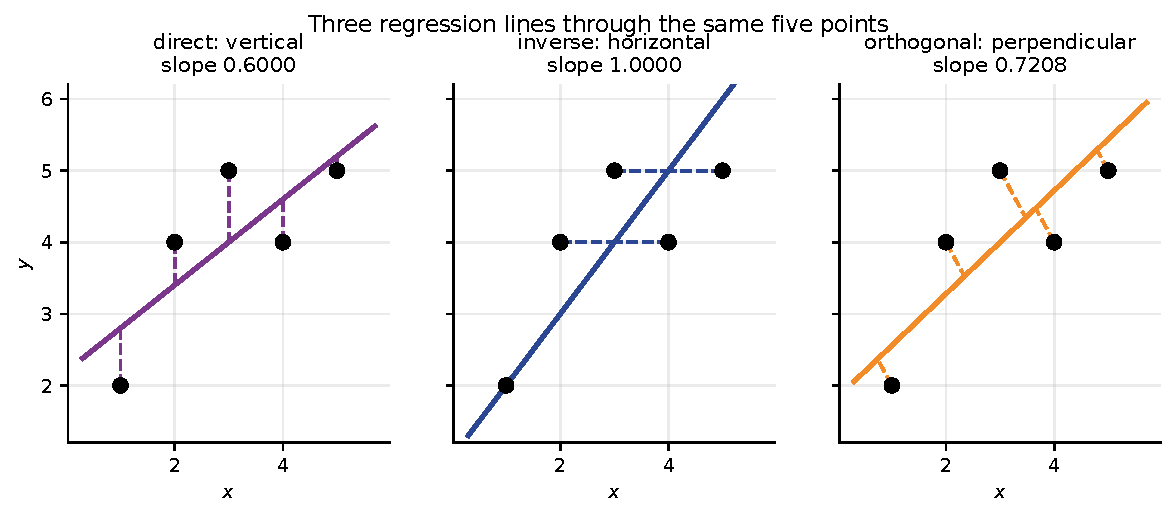
\includegraphics[width=0.80\textwidth]{direct.pdf}
\caption{The three methods on the same five points. The dashed segments are
the distances each method squares and adds. Every line passes through
$(\bar x, \bar y) = (3,4)$.}
\label{fig:direct}
\end{figure}

\subsection{The relationship between the two least-squares slopes}

The direct and inverse slopes are not independent. Writing
$b^{\mathrm{dir}} = S_{xy}/S_{xx}$ and $b^{\mathrm{inv}} = S_{yy}/S_{xy}$,
\[
  \frac{b^{\mathrm{dir}}}{b^{\mathrm{inv}}}
    = \frac{S_{xy}}{S_{xx}} \cdot \frac{S_{xy}}{S_{yy}}
    = \frac{S_{xy}^2}{S_{xx}S_{yy}}
    = r^2 .
\]
On our five points, $0.6/1.0 = 0.6 = r^2$. Two consequences worth stating.
First, the two slopes coincide \emph{only} when $r^2 = 1$, i.e.\ when the
points are exactly collinear. Second, for positive correlation the direct
slope is always the shallower of the two, and the orthogonal slope always lies
between them: $0.6000 < 0.7208 < 1.0000$.

\begin{caution}[Do not use the direct fit backwards]
If you fit $y$ on $x$ and then rearrange the equation to predict $x$ from $y$,
you have \emph{not} performed inverse regression. You have used the wrong
estimator: the correct inverse slope is $1.0$, and inverting the direct
equation gives $1/0.6 = 1.667$. The gap is the factor $1/r^2$, and it is large
exactly when the fit is weak.
\end{caution}

Each method minimises its own criterion and no other. This is worth measuring
rather than asserting.

\begin{lstlisting}
for name, s in [("direct", 0.6), ("inverse", 1.0), ("orthogonal", 0.7208)]:
    a = ybar - s * xbar
    r = y - (a + s * x)
    print(name, (r**2).sum(), (r**2).sum() / (1 + s*s), (r**2).sum() / (s*s))
\end{lstlisting}
\begin{codeout}
              vertical SS   perpendicular SS   horizontal SS
   direct        2.4000            1.7647          6.6667
   inverse       4.0000            2.0000          4.0000
   orthogonal    2.5458            1.6754          4.9006
\end{codeout}

Read down the diagonal: $2.4000$, $4.0000$, $1.6754$. Each is the smallest
number in its own column and in no other. There is no ``best line'' --- there
is a best line for a stated criterion. From here on, ``regression'' means the
direct method, and the next section explains why that criterion in particular.

% =========================================================================
\section{Maximum likelihood estimation}
\label{sec:mle}

\subsection{The question that least squares does not answer}

Why squares? The usual answers --- it is smooth, it has a closed form, it
punishes large errors --- are all true and all equally true of $\sum e_i^4$,
which has none of the properties we actually rely on. The real answer requires
a change of question. Instead of asking ``which line is closest?'', ask:

\begin{quote}
\emph{Suppose the data was generated by some random process with unknown
parameters. Which parameter values make the data I actually observed most
probable?}
\end{quote}

That is the \textbf{maximum likelihood} principle, and it is the single most
important idea in this unit. It will reappear unchanged in Lecture~10 for
logistic regression, where it produces cross-entropy rather than squares,
and again in Unit~VI for na\"ive Bayes.

\subsection{Step 0: the probability model}
\label{sec:model}

The model is one line of algebra and three assumptions:
\[
  y_i = \beta_0 + \beta_1 x_i + \varepsilon_i,
  \qquad
  \varepsilon_i \sim \mathcal{N}(0, \sigma^2)
  \quad\text{independently, for } i = 1,\dots,n .
\]
Equivalently, $y_i \sim \mathcal{N}(\beta_0 + \beta_1 x_i,\ \sigma^2)$. The
three assumptions, each of which Section~\ref{sec:adequacy} shows you how to
check:

\begin{enumerate}[leftmargin=*]
  \item \textbf{Linearity.} The \emph{mean} of $y$ at a given $x$ is
    $\beta_0 + \beta_1 x$. Not the value --- the mean.
  \item \textbf{Homoscedasticity.} The variance $\sigma^2$ is the
    \emph{same} at every $x$.
  \item \textbf{Independence and normality.} The $\varepsilon_i$ are
    independent draws from a Normal distribution.
\end{enumerate}

Note what is \emph{not} assumed: nothing about the distribution of $x$. The
$x_i$ are treated as fixed, known constants. That is the asymmetry of the
direct method, now stated as probability.

\begin{figure}[htbp]
\centering
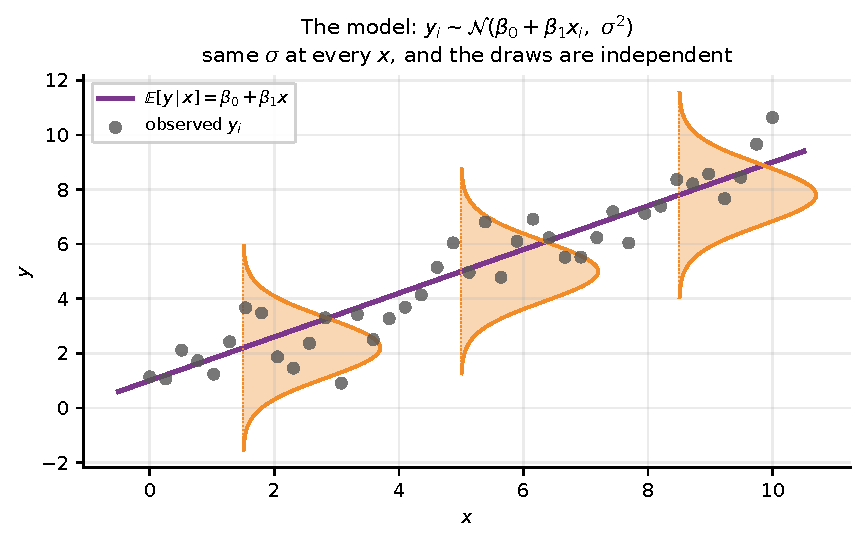
\includegraphics[width=0.56\textwidth]{mlegauss.pdf}
\caption{The line is the conditional mean; the orange bells are the
distribution of $y$ around it. Same width at every $x$ (assumption 2), and each
observation is one independent draw from its own bell.}
\label{fig:mlegauss}
\end{figure}

\subsection{Step 1: write the likelihood}

Write $e_i = y_i - \beta_0 - \beta_1 x_i$ for the error of observation $i$
at a candidate parameter value. Because $\varepsilon_i$ is Normal with mean
zero and variance $\sigma^2$, the density of the observation $y_i$ is
\[
  p(y_i \mid x_i,\, \beta_0,\, \beta_1,\, \sigma^2)
    = \frac{1}{\sqrt{2\pi\sigma^2}}
      \exp\!\left(-\frac{e_i^2}{2\sigma^2}\right).
\]
The $n$ observations are independent, so their joint density is the product of
the individual densities. Read as a function of the \emph{parameters} with the
data held fixed --- which is the reversal that gives the method its name ---
that product is the \textbf{likelihood}:
\begin{equation}
  L(\beta_0, \beta_1, \sigma^2)
    = \prod_{i=1}^{n} \frac{1}{\sqrt{2\pi\sigma^2}}
      \exp\!\left(-\frac{e_i^2}{2\sigma^2}\right)
    = \left(2\pi\sigma^2\right)^{-n/2}
      \exp\!\left(-\frac{1}{2\sigma^2}\sum_{i=1}^{n} e_i^2\right).
  \label{eq:lik}
\end{equation}
The second equality is only bookkeeping: $n$ copies of
$(2\pi\sigma^2)^{-1/2}$ multiply to $(2\pi\sigma^2)^{-n/2}$, and a product of
exponentials is the exponential of a sum. But look at what that sum is. The
sum of squared errors has appeared inside the exponent, and we have not chosen
anything yet.

\subsection{Step 2: take logarithms --- the central result}
\label{sec:central}

$\log$ is strictly increasing, so $\arg\max L = \arg\max \log L$: taking
logarithms cannot move the maximiser, and it turns the product into a sum.
Write $\ell = \log L$:
\begin{equation}
  \ell(\beta_0, \beta_1, \sigma^2)
    = -\frac{n}{2}\log(2\pi)
      \;-\; \frac{n}{2}\log \sigma^2
      \;-\; \frac{1}{2\sigma^2}\,
            \underbrace{\sum_{i=1}^{n}(y_i - \beta_0 - \beta_1 x_i)^2}
                       _{\textstyle S(\beta_0,\beta_1)} .
  \label{eq:loglik}
\end{equation}
Now read Equation~\eqref{eq:loglik} as a function of $\beta_0$ and $\beta_1$
alone, with $\sigma^2$ held at any fixed positive value.

\begin{itemize}[leftmargin=*]
  \item The first term, $-\tfrac{n}{2}\log(2\pi)$, is a constant.
  \item The second term, $-\tfrac{n}{2}\log\sigma^2$, does not involve
    $\beta_0$ or $\beta_1$ either.
  \item The third term is $-\dfrac{1}{2\sigma^2} S(\beta_0, \beta_1)$, where
    $1/(2\sigma^2) > 0$.
\end{itemize}

So $\ell$ is a positive constant times $-S$, plus a constant. Maximising a
negative multiple of $S$ is minimising $S$. Therefore, for every fixed
$\sigma^2 > 0$,
\begin{equation}
  \arg\max_{\beta_0,\beta_1} \ell(\beta_0,\beta_1,\sigma^2)
  \;=\;
  \arg\min_{\beta_0,\beta_1} S(\beta_0,\beta_1)
  \;=\;
  \arg\min_{\beta_0,\beta_1} \mathrm{SSE} .
  \label{eq:central}
\end{equation}

\begin{keyidea}[The central result of this lecture]
Under the assumption that the errors are independent Gaussian draws with a
common variance, \textbf{maximising the likelihood is exactly the same
optimisation problem as minimising the sum of squared errors}. Least squares
is therefore not an arbitrary convenience --- it is the maximum likelihood
estimator for a specific, checkable noise model. And because $\sigma^2$
appears only as a positive multiplier of $S$, the value of $\sigma^2$ cannot
change which line wins.
\end{keyidea}

Setting the derivatives of $S$ to zero now reproduces Lecture~8 exactly:
\[
  \frac{\partial S}{\partial \beta_0} = -2\sum_i e_i = 0,
  \qquad
  \frac{\partial S}{\partial \beta_1} = -2\sum_i x_i e_i = 0,
\]
which are the normal equations, with solution
$\hat\beta_1 = S_{xy}/S_{xx}$ and $\hat\beta_0 = \bar y - \hat\beta_1\bar x$.
\textbf{The estimator did not move. Its justification did}, and with it the
list of things you now have to check.

\begin{caution}[Two conclusions people wrongly draw from this]
\textbf{First}, this does \emph{not} say that your errors are Gaussian. It
says least squares is the ML estimator \emph{if} they are. Section~\ref{sec:laplace}
shows a case where they are not and the ML estimator is something else
entirely. \textbf{Second}, it does not say least squares is bad when the errors
are not Gaussian: by the Gauss--Markov theorem it remains the best
\emph{linear unbiased} estimator under much weaker conditions. What you lose is
the optimality among \emph{all} estimators, and every $p$-value.
\end{caution}

\subsection{Verifying the equivalence numerically}
\label{sec:verify}

The claim is that the two curves --- $\mathrm{SSE}$ against $b_1$, and $\ell$
against $b_1$ --- have their extrema in the same place, at every $\sigma^2$.
Take the five points and check.

\begin{lstlisting}
def loglik(b0, b1, s2):
    r = y - (b0 + b1 * x)
    return (-n/2*np.log(2*np.pi) - n/2*np.log(s2) - (r**2).sum() / (2*s2))

for g in [0.2, 0.4, 0.5, 0.6, 0.7, 0.8, 1.0]:
    a = ybar - g * xbar
    print(g, ((y - (a + g*x))**2).sum(), loglik(a, g, 0.48), loglik(a, g, 1.0))
\end{lstlisting}
\begin{codeout}
  b1     SSE      logL(sigma^2=0.48)   logL(sigma^2=1)
 0.20   4.0000         -6.926436        -6.594693
 0.40   2.8000         -5.676436        -5.994693
 0.50   2.5000         -5.363936        -5.844693
 0.60   2.4000         -5.259770        -5.794693
 0.70   2.5000         -5.363936        -5.844693
 0.80   2.8000         -5.676436        -5.994693
 1.00   4.0000         -6.926436        -6.594693
argmin SSE          b1 = 0.60000
argmax logL s2=0.48 b1 = 0.60000
argmax logL s2=1.00 b1 = 0.60000
closed form Sxy/Sxx b1 = 0.60000
\end{codeout}

Three things to notice. The SSE column is symmetric about $b_1 = 0.6$ --- it
is a parabola. The two log-likelihood columns contain \emph{different numbers}
($-5.2598$ against $-5.7947$ at the optimum), because $\sigma^2$ changes the
height and the curvature. And they peak in exactly the same place, to five
decimal places, which is Equation~\eqref{eq:central} measured.

\begin{figure}[htbp]
\centering
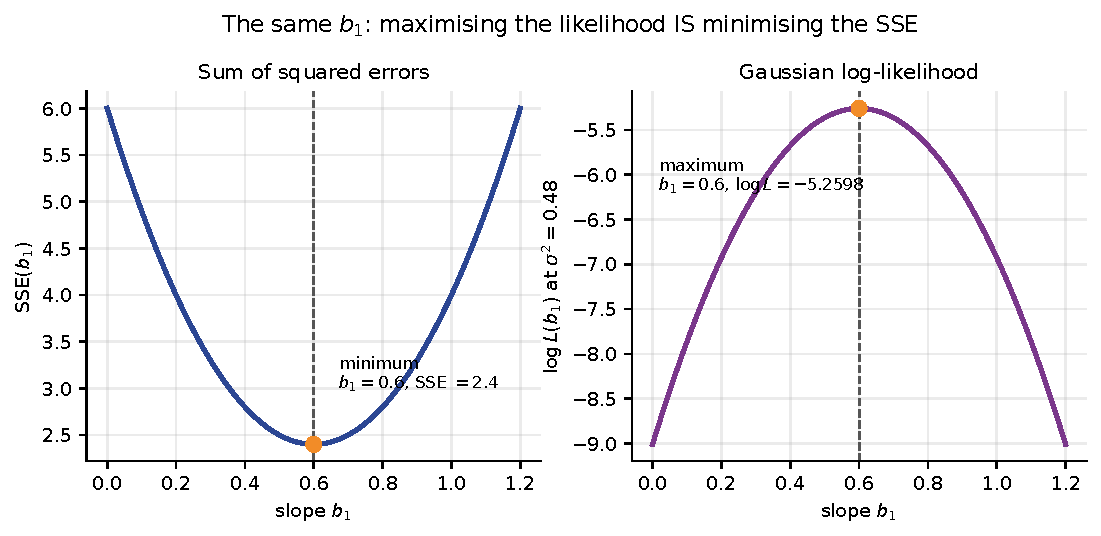
\includegraphics[width=0.68\textwidth]{mlecurve.pdf}
\caption{Left: SSE against the slope. Right: the log-likelihood at
$\sigma^2 = 0.48$ --- the same parabola, negated and shifted, with its maximum
in the same place, because $\ell = \text{const} - \mathrm{SSE}/(2\sigma^2)$.}
\label{fig:mlecurve}
\end{figure}

\subsection{Step 3: the maximum likelihood estimate of $\sigma^2$}
\label{sec:sigma}

The likelihood has a third parameter. Hold $\beta_0, \beta_1$ at their optimum
--- so that $\sum_i e_i^2 = \mathrm{SSE}$, a fixed number --- and differentiate
Equation~\eqref{eq:loglik} with respect to $\sigma^2$, treating $\sigma^2$ as
a single symbol $v$:
\[
  \ell = \text{const} - \frac{n}{2}\log v - \frac{\mathrm{SSE}}{2v},
  \qquad
  \frac{\partial \ell}{\partial v}
    = -\frac{n}{2v} + \frac{\mathrm{SSE}}{2v^2} = 0
  \quad\Longrightarrow\quad
  v = \frac{\mathrm{SSE}}{n}.
\]
So
\begin{equation}
  \hat\sigma^2_{\mathrm{ML}} = \frac{\mathrm{SSE}}{n}.
  \label{eq:sigmaml}
\end{equation}
The second derivative at that point is $-n^3/(2\,\mathrm{SSE}^2) < 0$, so it is
a maximum. Substituting Equation~\eqref{eq:sigmaml} back into
Equation~\eqref{eq:loglik} gives the maximised log-likelihood in closed form,
which is worth knowing because AIC and BIC are built from it:
\begin{equation}
  \ell_{\max}
    = -\frac{n}{2}\Bigl(\log\bigl(2\pi\hat\sigma^2_{\mathrm{ML}}\bigr) + 1\Bigr).
  \label{eq:lmax}
\end{equation}

\subsection{And this estimate is biased}
\label{sec:bias}

The slope and intercept MLEs are unbiased. The variance MLE is not.

The residuals $e_i = y_i - \hat y_i$ are not the errors $\varepsilon_i$: they
have been shrunk by the act of fitting. In matrix form
$\mathbf{e} = (I - H)\boldsymbol{\varepsilon}$, where $H$ is the hat matrix and
$\operatorname{tr}(I - H) = n - p$ with $p$ the number of estimated
coefficients ($p = 2$ for simple linear regression). Taking expectations,
\begin{equation}
  \mathbb{E}[\mathrm{SSE}] = (n - 2)\,\sigma^2
  \qquad\Longrightarrow\qquad
  \mathbb{E}\bigl[\hat\sigma^2_{\mathrm{ML}}\bigr]
    = \frac{n-2}{n}\,\sigma^2 \;<\; \sigma^2 .
  \label{eq:biased}
\end{equation}
The intuition is degrees of freedom. The residuals satisfy two exact linear
constraints --- $\sum_i e_i = 0$ and $\sum_i x_i e_i = 0$, both from the normal
equations --- so only $n-2$ of them are free to vary. Dividing a sum of $n-2$
free squares by $n$ understates the spread.

The unbiased estimator therefore divides by the degrees of freedom:
\begin{equation}
  s^2 = \frac{\mathrm{SSE}}{n-2},
  \qquad
  s = \sqrt{\frac{\mathrm{SSE}}{n-2}} \quad\text{(the \emph{standard error of
  the estimate})}.
  \label{eq:s2}
\end{equation}

\begin{worked}[The two estimates on the five points]
$\mathrm{SSE} = 2.4$ and $n = 5$, so
\[
  \hat\sigma^2_{\mathrm{ML}} = \frac{2.4}{5} = 0.48,
  \qquad
  s^2 = \frac{2.4}{3} = 0.80,
  \qquad
  s = 0.8944 .
\]
The ratio is $(n-2)/n = 3/5 = 0.6$: at $n = 5$ the maximum likelihood estimate
of the noise variance is \textbf{$40\%$ too small in expectation}. At $n = 100$
the same factor is $0.98$ and nobody notices --- but the small-sample case is
exactly the case in which you needed a variance estimate.
\end{worked}

\begin{lstlisting}
sse = ((y - yhat)**2).sum()
print(sse / n, sse / (n - 2), np.sqrt(sse / (n - 2)))
print(-n/2 * (np.log(2*np.pi*(sse/n)) + 1), loglik(b0, b1, sse/n))
\end{lstlisting}
\begin{codeout}
SSE            2.4000
sigma^2 MLE    = SSE/n     = 2.4000/5 = 0.4800
sigma^2 unbias = SSE/(n-2) = 2.4000/3 = 0.8000
ratio (n-2)/n  = 0.6000       s = sqrt(unbiased) = 0.8944
maximised log-likelihood = -n/2*(log(2*pi*s2_ml)+1) = -5.2598
direct evaluation                                   = -5.2598
\end{codeout}

The last two lines confirm Equation~\eqref{eq:lmax}: the closed form and the
direct evaluation of Equation~\eqref{eq:loglik} agree to four decimals.

\subsection{The bias is real: measuring it}
\label{sec:biasmeasured}

Equation~\eqref{eq:biased} is a statement about an average over datasets, so
generating many datasets is the way to check it. Simulate $20{,}000$ datasets
of $n = 10$ points from a known truth with $\sigma^2 = 4$, fit each, and record
both estimates.

\begin{lstlisting}
rng = np.random.default_rng(0)
xs = np.linspace(0, 9, 10)
for i in range(20000):
    ys = 1.0 + 2.0*xs + rng.normal(0, 2.0, 10)      # sigma^2 = 4
    b = ((xs-xs.mean())*(ys-ys.mean())).sum() / ((xs-xs.mean())**2).sum()
    e = ys - ((ys.mean() - b*xs.mean()) + b*xs)
    ml[i], unb[i] = (e**2).sum()/10, (e**2).sum()/8
\end{lstlisting}
\begin{codeout}
true sigma^2                    4.0000   (n = 10, 20000 replications)
mean of SSE/n     (the MLE)     3.2117   bias -0.7883
mean of SSE/(n-2) (unbiased)    4.0146   bias +0.0146
predicted MLE mean (n-2)/n*s^2  3.2000
the MLE was too small in 73.4% of the 20000 replications
\end{codeout}

The theory predicted $(n-2)/n \times 4 = 3.2000$ and the simulation returned
$3.2117$. That is not sampling noise: it is a systematic $20\%$ understatement,
and it occurred in nearly three runs out of four. A model that reports its own
noise as smaller than it is will also report prediction intervals narrower than
they should be, and confidence intervals for the coefficients that are too
tight.

\begin{figure}[htbp]
\centering
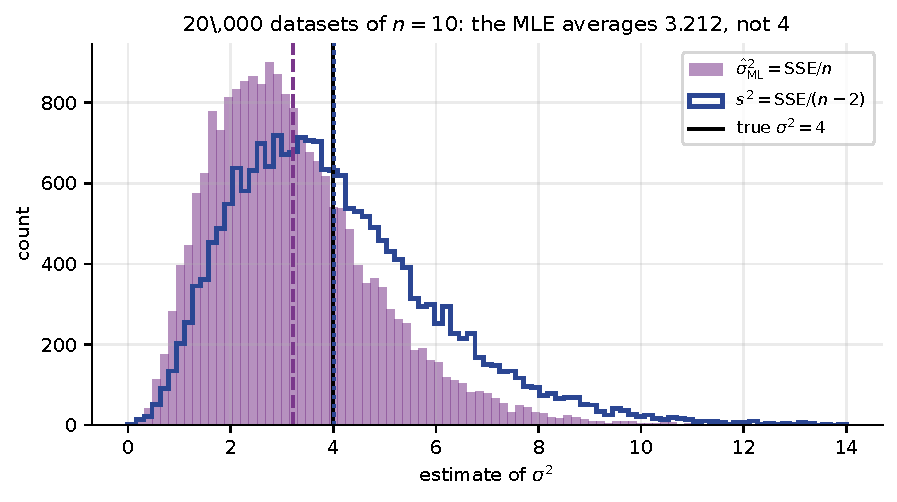
\includegraphics[width=0.56\textwidth]{sigmabias.pdf}
\caption{The same histogram stretched by $n/(n-2) = 1.25$; both are
right-skewed because $\mathrm{SSE}/\sigma^2$ is $\chi^2_{n-2}$. Unbiased does
not mean accurate --- at $n = 10$ both estimators are wildly variable.}
\label{fig:sigmabias}
\end{figure}

\begin{caution}[``Unbiased'' is a statement about an average, not about your dataset]
$s^2 = 4.0146$ is the mean over $20{,}000$ datasets. On any \emph{one} dataset
of ten points the estimate ranged over an order of magnitude. Do not read
unbiasedness as reliability.
\end{caution}

\subsection{Change the noise model, and the estimator changes}
\label{sec:laplace}

If maximum likelihood is what justifies least squares, then a different noise
distribution must justify a different criterion. It does, and this is the
sharpest way to see that the Gaussian assumption is doing real work.

Suppose $\varepsilon_i$ follows a Laplace (double exponential) distribution
with density $\tfrac{1}{2b}\exp(-|e|/b)$. Then
\[
  \ell = -n\log(2b) - \frac{1}{b}\sum_{i=1}^{n} |e_i|,
\]
and maximising it means minimising $\sum_i |e_i|$ --- \textbf{least absolute
deviations}, not least squares. The recipe is the same; only the answer
changes.

\begin{lstlisting}
rng = np.random.default_rng(0)             # the one seed for this lecture
xl = np.linspace(0, 10, 60)
yl = 2.0 + 1.5*xl + rng.laplace(0, 1.0, 60);  yl[13] += 25.0
ols = np.polyfit(xl, yl, 1)
lad = minimize(lambda p: np.abs(yl - (p[0] + p[1]*xl)).sum(), [0., 1.],
               method="Nelder-Mead").x
\end{lstlisting}
\begin{codeout}
true intercept 2.0000  true slope 1.5000
Gaussian MLE  = least squares    : intercept 3.0024  slope 1.3738
Laplace  MLE  = least abs. dev.  : intercept 2.7650  slope 1.3730
sum of squared residuals  OLS 622.2965   LAD 625.7886
sum of |residuals|        OLS 85.8123   LAD 83.6585
\end{codeout}

Each estimator wins its own criterion: OLS has the smaller
$\sum e_i^2$ ($622.30 < 625.79$) and LAD the smaller $\sum|e_i|$
($83.66 < 85.81$). Neither is cheating --- each is minimising exactly what it
was asked to minimise, and each therefore loses on the other's scoreboard.

Now compare them to the truth, $(\beta_0, \beta_1) = (2.0, 1.5)$. LAD
recovered the intercept as $2.77$ against OLS's $3.00$, so the outlier drags
least squares further. The two \emph{slopes}, though, are for practical
purposes identical on this draw: $1.3730$ against $1.3738$. Be honest about
that. A single dataset of sixty points is nowhere near enough to display an
efficiency difference between two consistent estimators; what it displays is
that one heavy draw moves both fits away from the truth, and moves the
squared-error fit further.

\begin{caution}[What this example does and does not show]
It shows that the criterion you minimise is a \emph{modelling choice} that
follows from the noise distribution you assume --- Gaussian gives squares,
Laplace gives absolute values --- and that the two choices give genuinely
different answers on the same data. It does \emph{not} show that LAD is
reliably more accurate, and one run of one dataset could not show that. If you
want that claim, you need many replications, which is precisely the design of
the simulation in Section~\ref{sec:biasmeasured}. Do not over-read a single
sample.
\end{caution}

\begin{keyidea}
The recipe is: state the noise distribution, write the likelihood, take
logarithms, maximise. Gaussian noise gives squares. Laplace noise gives
absolute values. In Lecture~10, a Bernoulli response will give cross-entropy.
\textbf{Learn the recipe, not the formula it happens to produce here.}
\end{keyidea}

\begin{tryit}
Show by hand that for a \emph{single} parameter --- fitting only a constant,
$y_i = \mu + \varepsilon_i$ --- the Gaussian MLE of $\mu$ is the sample mean
and the Laplace MLE is the sample median. Then check numerically on
$y = (1, 2, 3, 4, 100)$: you should get $\hat\mu_{\text{Gauss}} = 22.0$ and
$\hat\mu_{\text{Laplace}} = 3.0$. That single number is the whole argument for
robust regression.
\end{tryit}

% =========================================================================
\section{The coefficient of determination}
\label{sec:r2}

\subsection{What $R^2$ compares}

Having fitted a line, you want one number for how good it is. $R^2$ answers a
specific comparative question: \emph{how much better is my line than the flat
line $\hat y = \bar y$?}

Start from the identity, valid whenever the model contains an intercept:
\begin{equation}
  \underbrace{\sum_i (y_i - \bar y)^2}_{\mathrm{SS_{tot}}}
  =
  \underbrace{\sum_i (\hat y_i - \bar y)^2}_{\mathrm{SS_{reg}}}
  +
  \underbrace{\sum_i (y_i - \hat y_i)^2}_{\mathrm{SS_{res}}} .
  \label{eq:decomp}
\end{equation}
It follows from writing $y_i - \bar y = (\hat y_i - \bar y) + (y_i - \hat y_i)$
and squaring: the cross term is
$2\sum_i (\hat y_i - \bar y)e_i = 2\bigl(\hat\beta_0\sum_i e_i +
\hat\beta_1 \sum_i x_i e_i - \bar y \sum_i e_i\bigr) = 0$, because the normal
equations force $\sum_i e_i = 0$ and $\sum_i x_i e_i = 0$. Then
\begin{equation}
  R^2 = 1 - \frac{\mathrm{SS_{res}}}{\mathrm{SS_{tot}}}
      = \frac{\mathrm{SS_{reg}}}{\mathrm{SS_{tot}}} .
  \label{eq:r2}
\end{equation}

\begin{caution}[The decomposition needs the intercept]
Fit without an intercept and $\sum_i e_i \ne 0$, the cross term does not
vanish, Equation~\eqref{eq:decomp} fails, and the two expressions in
Equation~\eqref{eq:r2} stop agreeing. Different software then reports
different ``$R^2$'' for the same no-intercept fit. If you ever need a
no-intercept model, report the residual standard error instead.
\end{caution}

\subsection{Worked: the whole calculation on five rows}
\label{sec:r2hand}

\begin{worked}[$R^2$ from the definition]
The five points again, with $\hat y = 2.2 + 0.6x$.
\begin{center}
\begin{tabular}{@{}rrrrrrr@{}}
\toprule
$x$ & $y$ & $\hat y$ & $y-\bar y$ & $(y-\bar y)^2$ & $y - \hat y$ & $(y-\hat y)^2$\\
\midrule
$1$ & $2$ & $2.8$ & $-2.0$ & $4.00$ & $-0.8$ & $0.64$\\
$2$ & $4$ & $3.4$ & $ 0.0$ & $0.00$ & $ 0.6$ & $0.36$\\
$3$ & $5$ & $4.0$ & $ 1.0$ & $1.00$ & $ 1.0$ & $1.00$\\
$4$ & $4$ & $4.6$ & $ 0.0$ & $0.00$ & $-0.6$ & $0.36$\\
$5$ & $5$ & $5.2$ & $ 1.0$ & $1.00$ & $-0.2$ & $0.04$\\
\midrule
& & & & $\mathrm{SS_{tot}} = 6.00$ & & $\mathrm{SS_{res}} = 2.40$\\
\bottomrule
\end{tabular}
\end{center}
\[
  R^2 = 1 - \frac{2.40}{6.00} = 0.6000,
  \qquad
  s = \sqrt{\frac{2.40}{5-2}} = \sqrt{0.8} = 0.8944 .
\]
Two independent checks. First, $\mathrm{SS_{reg}} = 6.00 - 2.40 = 3.60$, and
separately $b_1^2 S_{xx} = 0.36 \times 10 = 3.60$. Second,
$r = S_{xy}/\sqrt{S_{xx}S_{yy}} = 6/\sqrt{60} = 0.7746$ and $r^2 = 0.6000$.
\end{worked}

\begin{figure}[htbp]
\centering
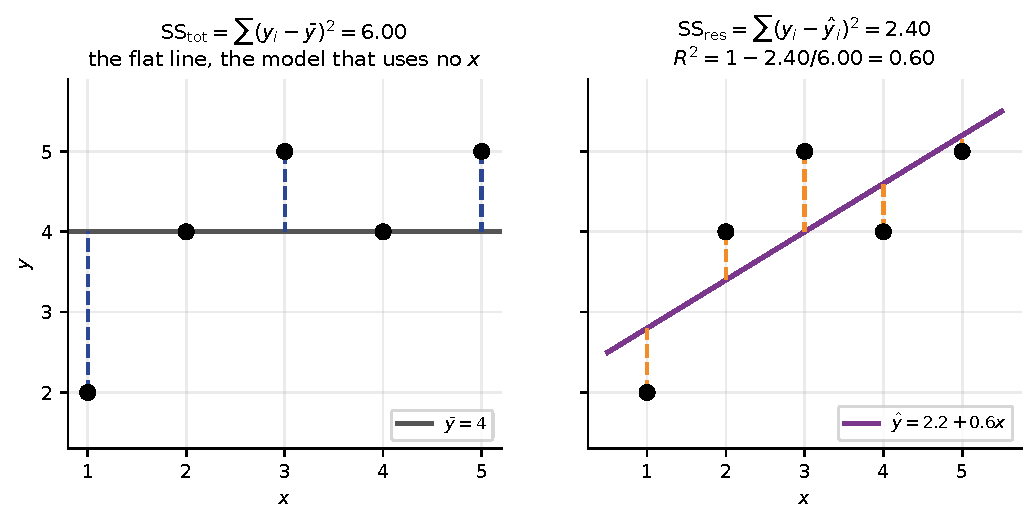
\includegraphics[width=0.68\textwidth]{r2hand.pdf}
\caption{Left: deviations from $\bar y = 4$, squaring and adding to $6.00$.
Right: deviations from the fitted line, adding to $2.40$. $R^2$ is the fraction
of the left picture that the right picture removed.}
\label{fig:r2hand}
\end{figure}

\subsection{Three identities worth knowing}

For \emph{simple} linear regression --- one predictor plus an intercept ---
the following are all the same number:
\begin{equation}
  R^2 \;=\; 1 - \frac{\mathrm{SS_{res}}}{\mathrm{SS_{tot}}}
      \;=\; \frac{\mathrm{SS_{reg}}}{\mathrm{SS_{tot}}}
      \;=\; \frac{b_1^2 S_{xx}}{S_{yy}}
      \;=\; r^2
      \;=\; \operatorname{corr}(y, \hat y)^2 .
  \label{eq:ident}
\end{equation}
The last of these is the one that generalises: with several predictors, $r^2$
of any single predictor is no longer $R^2$, but the squared correlation
between $y$ and the fitted values still is.

\begin{lstlisting}
from sklearn.metrics import r2_score
print(r2_score(y, yhat))
print(LinearRegression().fit(x[:, None], y).score(x[:, None], y))
\end{lstlisting}
\begin{codeout}
SSreg = SStot - SSres = 3.60      b1^2 * Sxx = 3.60
R2 = 1 - SSres/SStot = 1 - 2.40/6.00 = 0.6000
r^2 = (Sxy/sqrt(Sxx*Syy))^2 = 0.6000
sklearn r2_score            = 0.6000
s = sqrt(SSres/(n-2))       = 0.8944
\end{codeout}

Four routes to the same $0.6000$. \texttt{r2\_score} is three lines of
arithmetic, not a verdict, and the rest of this section is about what those
three lines cannot see.

\subsection{$R^2$ never decreases when you add a predictor}
\label{sec:noisecols}

Here is the property that makes a reported $R^2$ untrustworthy as a measure of
model quality.

\begin{keyidea}
Adding a column to a linear model can never decrease its training $R^2$, no
matter what is in the column. The old fit is still available in the enlarged
model --- just set the new coefficient to zero --- so the minimised
$\mathrm{SS_{res}}$ can only stay the same or fall.
\end{keyidea}

The argument is one sentence, and it is worth checking that reality obeys it.
Take $30$ rows with one genuine predictor, and append columns of
$\mathcal{N}(0,1)$ noise generated \emph{without ever looking at} $y$.

\begin{lstlisting}
rng = np.random.default_rng(0)             # the one seed for this lecture
xr = rng.normal(0, 1, 30)
yr = 1.0 + 2.0*xr + rng.normal(0, 2.0, 30)
noise = rng.normal(0, 1, (30, 27))
for k in range(28):
    X = np.c_[xr, noise[:, :k]]
    print(k, LinearRegression().fit(X, yr).score(X, yr))
\end{lstlisting}
\begin{codeout}
  extra noise columns   p   R2        adjusted R2
         0             1   0.241296   +0.214199
         1             2   0.258852   +0.203952
         2             3   0.344538   +0.268908
         5             6   0.402777   +0.246979
        10            11   0.660344   +0.452777
        15            16   0.743023   +0.426743
        20            21   0.793909   +0.252920
        25            26   0.852039   -0.430293
        27            28   0.940085   -0.737539
R2 decreased at any step?  False   (28 nested models)
smallest single-step change +0.00000315
R2 with 27 pure-noise columns and 30 rows: 0.940085
\end{codeout}

$R^2$ went from $0.2413$ to $0.9401$ and \emph{never once fell}: the smallest
single step across all $27$ additions was $+3\times10^{-6}$, on the positive
side. Extrapolating, at $p = 29$ the model would have as many parameters as
rows and $R^2$ would be exactly $1$.

\begin{caution}[What this rules out]
$R^2$ cannot be used to compare models of different sizes, and ``we added
features and $R^2$ went up'' is not evidence of anything. It is a theorem.
\end{caution}

\subsection{Adjusted $R^2$, and how far it gets you}
\label{sec:adjr2}

The standard correction charges you for each parameter:
\begin{equation}
  R^2_{\mathrm{adj}} = 1 - (1 - R^2)\,\frac{n-1}{n-p-1},
  \label{eq:adj}
\end{equation}
where $p$ is the number of predictors excluding the intercept. Equivalently,
it replaces the two sums of squares by their mean squares:
$1 - \dfrac{\mathrm{SS_{res}}/(n-p-1)}{\mathrm{SS_{tot}}/(n-1)}$. Unlike
$R^2$, it can fall when a useless column is added, and it can be negative.

On the $30$-row experiment it worked perfectly: $+0.2142$ at $p = 1$ and
$\mathbf{-0.7375}$ at $p = 28$. Now try the same trick on real data, where $n$
is large.

\begin{lstlisting}
rng = np.random.default_rng(0)             # the one seed for this lecture
NOISE = rng.normal(0, 1, (442, 400))
for k in [0, 10, 50, 100, 200, 300, 400]:
    X = np.c_[Xd, NOISE[:, :k]]
    m = LinearRegression().fit(X, yd)
    cv = cross_val_score(LinearRegression(), X, yd,
                         cv=KFold(5, shuffle=True, random_state=0), scoring="r2")
\end{lstlisting}
\begin{codeout}
load_diabetes: 442 rows, 10 real features
  noise cols    p     R2        adjusted R2   5-fold CV R2
       0        10   0.517748   +0.506559     +0.489155
      10        20   0.538221   +0.516283     +0.488619
      50        60   0.592908   +0.528799     +0.424743
     100       110   0.643486   +0.525008     +0.337363
     200       210   0.759013   +0.539935     -0.105104
     300       310   0.887148   +0.620092     -1.980381
     400       410   0.976075   +0.659652     -5.760536
\end{codeout}

Read the last row. With $410$ pure-noise columns on $442$ patients, $R^2$ is
$0.9761$, adjusted $R^2$ is $+0.6597$ --- \emph{higher} than it was with no
noise at all --- and the cross-validated $R^2$ is $-5.7605$.

\begin{keyidea}
Adjusted $R^2$ is a penalty, not a test. On a small dataset it caught a
fabricated model completely; on a larger one it was still reporting $+0.54$
while the model's actual predictive value was catastrophically negative.
\textbf{Report adjusted $R^2$ if you like; trust the number computed on rows
the fit never saw.}
\end{keyidea}

\begin{figure}[htbp]
\centering
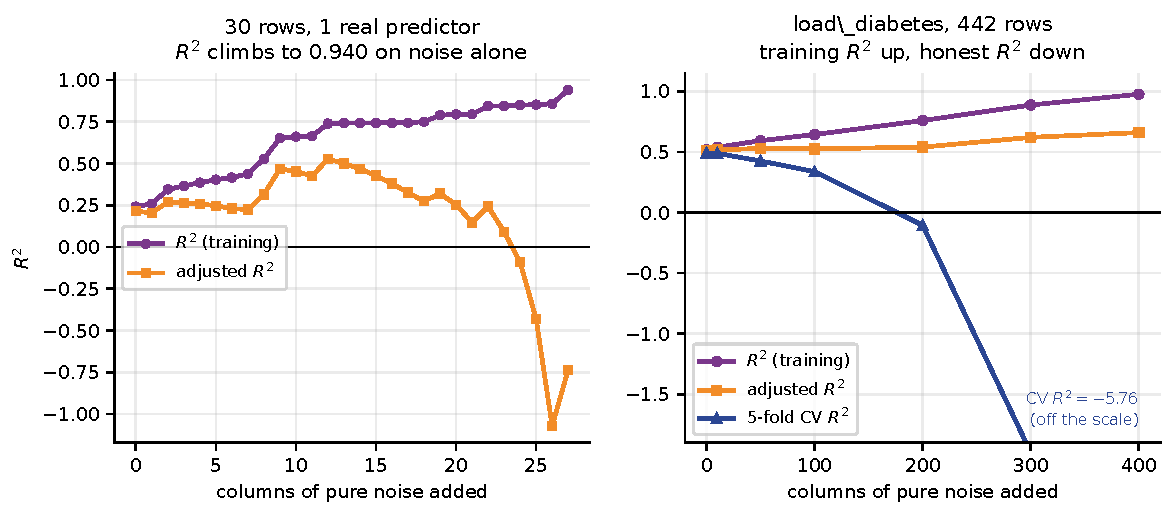
\includegraphics[width=0.80\textwidth]{r2noise.pdf}
\caption{Left, $30$ rows: $R^2$ climbs to $0.908$ on noise while adjusted
$R^2$ collapses to $-1.66$. Right, $442$ rows: $R^2$ climbs, adjusted $R^2$
stays flat and complacent near $0.5$, and cross-validated $R^2$ falls off the
bottom of the chart. Only the third curve is measuring prediction.}
\label{fig:r2noise}
\end{figure}

\subsection{$R^2$ can be negative}
\label{sec:negr2}

$R^2 \in [0,1]$ is only guaranteed \emph{on the data the intercept was fitted
to}. There, the flat line $\hat y = \bar y$ is one of the fits available to the
model, so the minimised $\mathrm{SS_{res}}$ cannot exceed $\mathrm{SS_{tot}}$.
On held-out data no such guarantee exists: $\bar y_{\mathrm{test}}$ is a number
the model has never seen.

\begin{worked}[Negative $R^2$ in three numbers]
Held-out values $y = (1, 2, 3)$; the model predicts $(3, 2, 1)$.
$\bar y_{\mathrm{test}} = 2$, so
\[
  \mathrm{SS_{tot}} = 1 + 0 + 1 = 2,
  \qquad
  \mathrm{SS_{res}} = 4 + 0 + 4 = 8,
  \qquad
  R^2 = 1 - \frac{8}{2} = -3 .
\]
Predicting the constant $2$ for all three would have given $R^2 = 0$. There is
no lower bound at all: scale the predictions up and $R^2 \to -\infty$.
\end{worked}

\begin{lstlisting}
print(r2_score([1., 2., 3.], [3., 2., 1.]))
print(r2_score([1., 2., 3.], [2., 2., 2.]))
\end{lstlisting}
\begin{codeout}
y_test       [1. 2. 3.]
prediction   [3. 2. 1.]
mean of y_test 2.0000  SStot 2.0000  SSres 8.0000
R2 = 1 - 8.0/2.0 = -3.0000     sklearn -3.0000
R2 of the constant prediction 2.0: 0.0000
\end{codeout}

This is not a contrived edge case. It is the routine outcome of an over-fitted
model, as the next section will show at length.

\begin{lstlisting}
c = np.polynomial.Polynomial.fit(x_train, y_train, 14)   # 25 training points
print(r2_score(y_train, c(x_train)), r2_score(y_test, c(x_test)))
\end{lstlisting}
\begin{codeout}
degree   train R2    test R2
   3     +0.894255  +0.875699
   9     +0.918465  +0.838709
  14     +0.953629  -1.105552
  18     +0.959084  -2864.487739
  22     +0.965154  -1532443280.011133
\end{codeout}

\begin{figure}[htbp]
\centering
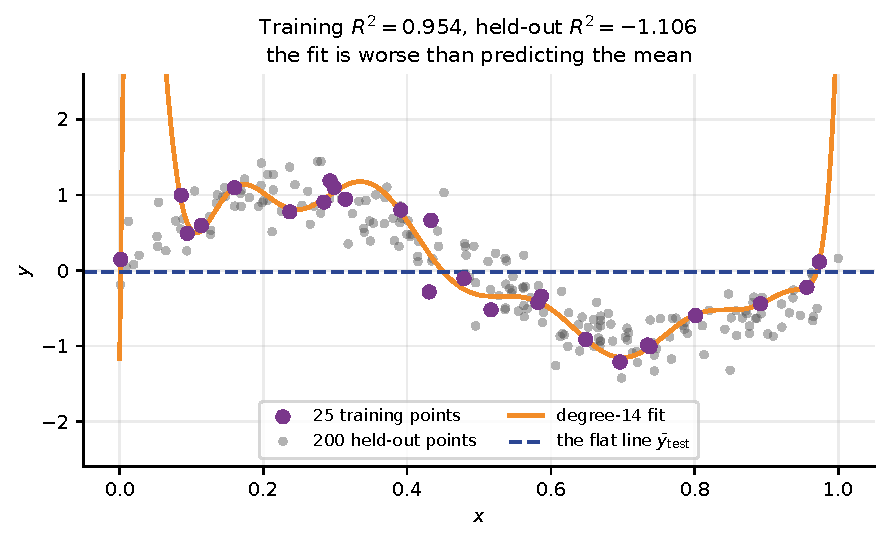
\includegraphics[width=0.56\textwidth]{r2negative.pdf}
\caption{Training $R^2 = 0.954$, held-out $R^2 = -1.106$. The curve passes
beautifully close to every training point and leaves the data entirely between
them. The blue dashed line --- predict the mean and go home --- beats it.}
\label{fig:r2neg}
\end{figure}

\begin{keyidea}
A negative held-out $R^2$ is not a bug and not a rounding error. It means the
model is worse than a constant. Whenever you see one, the honest report is
``this model has no predictive value on this data''.
\end{keyidea}

% =========================================================================
\section{Checking model adequacy}
\label{sec:adequacy}

\subsection{What one number cannot see}

$R^2$ is a ratio of two sums. It has no access to the \emph{order} of the
residuals, their \emph{shape}, or their \emph{pattern against} $\hat y$. Every
assumption of Section~\ref{sec:model} can fail while $R^2$ stays high.

\begin{center}
\begin{tabular}{@{}lp{5.4cm}p{4.7cm}@{}}
\toprule
\textbf{Assumption} & \textbf{How it fails} & \textbf{What it invalidates}\\
\midrule
Linearity & residuals versus fitted show an arch or a U &
  the coefficients themselves; the model is simply wrong\\[4pt]
Constant variance & the residual cloud fans out with $\hat y$ &
  standard errors, $p$-values, all intervals\\[4pt]
Normality & Q--Q plot bends at the ends &
  $p$-values and intervals in small samples\\[4pt]
Independence & residuals plotted in order drift or oscillate &
  standard errors, badly; often understates them\\[4pt]
No single point in charge & one row has leverage near $1$ &
  everything: delete the row and the fit moves\\
\bottomrule
\end{tabular}
\end{center}

\subsection{Anscombe's quartet}
\label{sec:anscombe}

In 1973 F.\ J.\ Anscombe published four datasets of eleven points each,
constructed to share almost every summary statistic. Lecture~8 used them to
make the point that a table of numbers is not a substitute for a plot; here we
take the next step and read the \emph{residuals}, which turn ``these look
different'' into four separate, nameable diagnoses. The data is short enough to
type out.

\begin{lstlisting}
x123 = [10., 8., 13., 9., 11., 14., 6., 4., 12., 7., 5.]
y1 = [8.04, 6.95, 7.58, 8.81, 8.33, 9.96, 7.24, 4.26, 10.84, 4.82, 5.68]
y2 = [9.14, 8.14, 8.74, 8.77, 9.26, 8.10, 6.13, 3.10, 9.13, 7.26, 4.74]
y3 = [7.46, 6.77, 12.74, 7.11, 7.81, 8.84, 6.08, 5.39, 8.15, 6.42, 5.73]
x4 = [8., 8., 8., 8., 8., 8., 8., 19., 8., 8., 8.]
y4 = [6.58, 5.76, 7.71, 8.84, 8.47, 7.04, 5.25, 12.50, 5.56, 7.91, 6.89]
\end{lstlisting}
\begin{codeout}
set  mean x  mean y   sd x    sd y   intercept  slope    R2      SSres
I     9.000   7.501   3.317   2.032    3.0001  0.5001  0.6665  13.7627
II    9.000   7.501   3.317   2.032    3.0009  0.5000  0.6662  13.7763
III   9.000   7.500   3.317   2.030    3.0025  0.4997  0.6663  13.7562
IV    9.000   7.501   3.317   2.031    3.0017  0.4999  0.6667  13.7425
\end{codeout}

Identical means, identical standard deviations, the same fitted line
$\hat y = 3.00 + 0.50x$, the same $R^2 = 0.666$ and the same residual sum of
squares to two decimals. Anyone reading only that table would conclude these
are four samples from the same population.

\begin{figure}[htbp]
\centering

\includegraphics[width=0.54\textwidth]{anscombe.pdf}
\caption{I is a genuine noisy line; II an exact parabola (wrong model, not
noisy data); III a perfect line with one contaminated point; IV ten points at
$x = 8$ and one at $x = 19$, which alone determines the slope.}
\label{fig:anscombe}
\end{figure}

\subsection{The residual plot gives four different diagnoses}
\label{sec:resplot}

Plotting the residuals $e_i = y_i - \hat y_i$ against the fitted values
$\hat y_i$ is the single most informative diagnostic in regression. A model
that fits well produces a shapeless horizontal band. Anything else is a
message.

\begin{figure}[htbp]
\centering
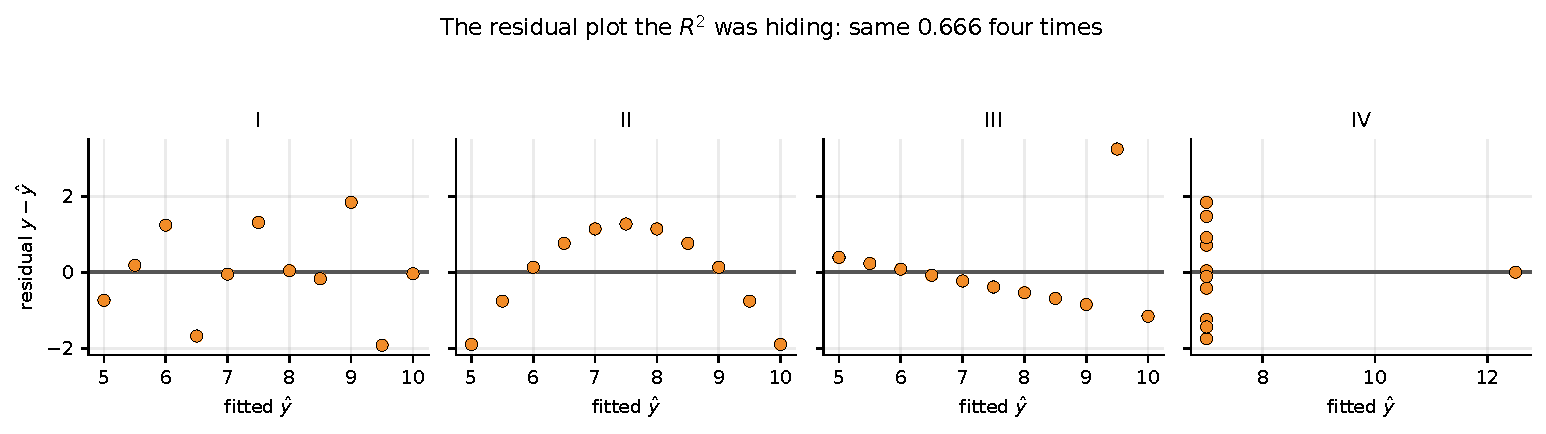
\includegraphics[width=0.80\textwidth]{ansresid.pdf}
\caption{Residuals against fitted values for the four Anscombe datasets. Same
$R^2 = 0.666$; four different pictures.}
\label{fig:ansresid}
\end{figure}

Four numeric diagnostics separate them completely. \emph{Curvature} $R^2$ is
what a parabola fitted to the residuals explains. \emph{Leverage} is
$h_i = 1/n + (x_i - \bar x)^2 / S_{xx}$, the influence of row $i$ on its own
fitted value; it sums to $p = 2$, so an average row has $h \approx 0.18$ here.

\begin{lstlisting}
e = ya - (ic + sl * xa)
curv = r2_score(e, np.polyval(np.polyfit(xa, e, 2), xa))
h = 1/len(xa) + (xa - xa.mean())**2 / ((xa - xa.mean())**2).sum()
\end{lstlisting}
\begin{codeout}
set  max|e|  |e|max/|e|2nd  curvature R2  Shapiro p  max leverage  slope w/o pt
I     1.921           1.04        0.0623     0.5456        0.3182        0.5028
II    1.901           1.00        1.0000     0.0929        0.3182        0.6267
III   3.241           2.80        0.0550     0.0016        0.3182        0.5770
IV    1.839           1.05        0.0000     0.7800        1.0000     undefined
\end{codeout}

\begin{itemize}[leftmargin=*]
  \item \textbf{I} --- nothing stands out. Curvature $R^2 = 0.06$, largest
    residual barely bigger than the next, Shapiro $p = 0.55$, leverage $0.32$.
    Deleting the highest-leverage point moves the slope from $0.5001$ to
    $0.5028$. This is what an adequate model looks like.
  \item \textbf{II} --- a parabola fitted to the residuals explains
    \textbf{$100.00\%$} of them. There is no noise left, only unmodelled
    curvature: the correct model is quadratic, and the linear fit's
    ``residuals'' are entirely signal.
  \item \textbf{III} --- the largest residual is $2.80\times$ the next, and
    Shapiro rejects normality at $p = 0.0016$. Ten of the eleven points lie
    exactly on a line; one does not. The fitted slope of $0.4997$ belongs to
    neither the ten nor the one.
  \item \textbf{IV} --- leverage $\mathbf{1.0000}$. One point supplies the
    entire spread of $x$, so it fixes its own fitted value exactly, and
    deleting it leaves the slope \textbf{undefined} (all remaining $x$ are
    equal). There is no evidence for linearity here at all.
\end{itemize}

\begin{keyidea}
The same $R^2$ described a good fit, a wrong model, a contaminated dataset and
a fit with no evidence behind it. \textbf{Never report an $R^2$ without a
residual plot beside it.}
\end{keyidea}

\subsection{Non-constant variance, measured}
\label{sec:hetero}

Heteroscedasticity --- variance changing with $x$ or $\hat y$ --- is the
commonest violation in practice, because so many real quantities have noise
proportional to their size. Construct a case where the noise sd grows linearly
with $x$.

\begin{lstlisting}
rng = np.random.default_rng(0)             # the one seed for this lecture
xh = np.sort(rng.uniform(1, 10, 200))
yh = 3.0 + 2.0*xh + rng.normal(0, 1, 200) * (0.25*xh)     # sd grows with x
eh = yh - np.polyval(np.polyfit(xh, yh, 1), xh)
aux = LinearRegression().fit(fh.reshape(-1, 1), eh**2)    # Breusch-Pagan
lm = len(xh) * aux.score(fh.reshape(-1, 1), eh**2)
\end{lstlisting}
\begin{codeout}
fit: intercept 2.8790  slope 2.0011   R2 0.9267
residual sd, lower half of x  1.0460
residual sd, upper half of x  1.8988   ratio 1.82
Breusch-Pagan LM = n*R2(e^2 on yhat) = 22.9065   chi2(1) p = 0.000002
Shapiro-Wilk on the residuals p = 0.031073
after log(y): Breusch-Pagan LM = 3.2426   p = 0.0717   sd ratio 0.89
\end{codeout}

$R^2 = 0.9267$, which most people would call a good fit. The residual standard
deviation over the upper half of $x$ is $1.82\times$ that over the lower half,
and the Breusch--Pagan test --- regress the squared residuals on the fitted
values and compare $nR^2$ to a $\chi^2_1$ --- returns $22.91$ with
$p \approx 2\times10^{-6}$. The variance is not constant, and no amount of
$R^2$ was ever going to say so.

Note the fourth line honestly: the Shapiro--Wilk test also rejects, but only
just, at $p = 0.031073$. Non-constant variance shows up as apparent
non-normality, because a mixture of Normals with different variances is not
Normal --- but it shows up \emph{weakly}, because that mixture is still
symmetric and unimodal. That is the useful lesson: the test that is aimed at
the actual defect ($p \approx 2\times10^{-6}$) is three decimal orders more
decisive than the test that is not ($p = 0.031$). The two diagnostics are not
independent, and the residual plot is what tells you which problem you
actually have.

\begin{figure}[htbp]
\centering
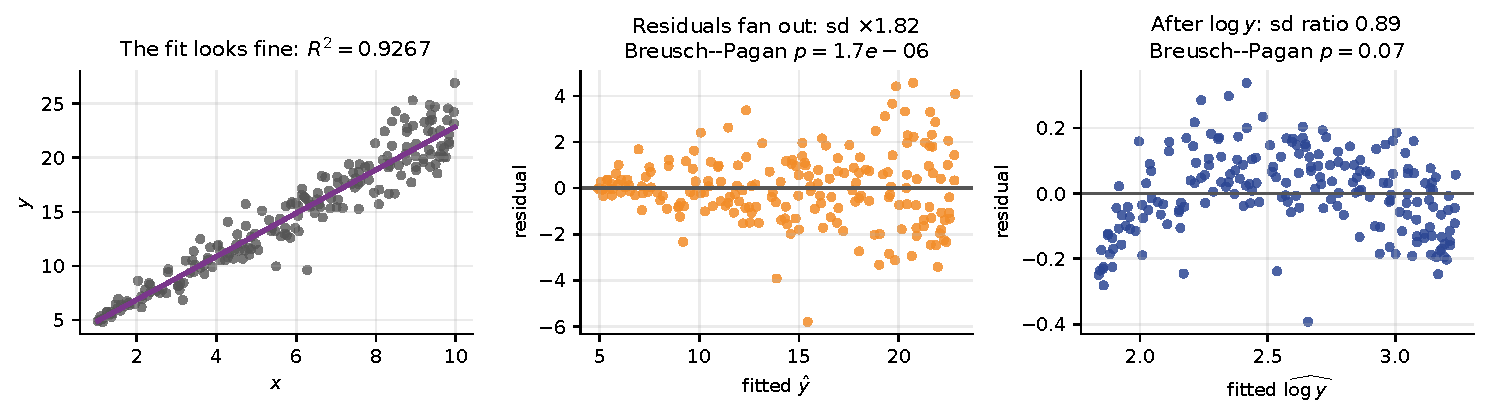
\includegraphics[width=0.80\textwidth]{hetero.pdf}
\caption{Left, the plot you would put in a report. Middle, the plot that tells
the truth: a wedge, wide on the right. Right, the same data after $\log y$ ---
much closer to a shapeless band, which is what a residual plot should look
like, though the transform has not removed the effect entirely.}
\label{fig:hetero}
\end{figure}

\begin{caution}[What heteroscedasticity does and does not break]
It does \textbf{not} bias the coefficients: least squares stays unbiased
without any constant-variance assumption. What it breaks is everything
downstream --- standard errors, $t$ and $F$ statistics, $p$-values,
confidence and prediction intervals --- because all of them are computed as if
$\sigma$ were a single number. Taking $\log y$ here moved the test statistic
from $22.91$ to $3.24$, and its $p$-value from $2\times10^{-6}$ to $0.072$ ---
a large improvement, but not a clean bill of health. A transform is a remedy
to be checked, not a box to be ticked.
\end{caution}

\subsection{The normal Q--Q plot}
\label{sec:qq}

Sort the residuals and plot them against the quantiles they would occupy if
they were Gaussian. A straight line means the residuals are Normal; departures
at the ends are what matter.

\begin{lstlisting}
q = stats.norm.ppf((np.arange(1, n+1) - 0.5) / n)
plt.scatter(q, np.sort(e - e.mean()))
\end{lstlisting}
\begin{codeout}
residual model     corr(ordered resid, normal quantile)   Shapiro p   kurtosis
Gaussian noise                              0.9935    0.198668    -0.5004
t(3) noise                                  0.9626    0.000009     2.7920
uniform noise                               0.9845    0.003336    -1.0901
\end{codeout}

\begin{figure}[htbp]
\centering
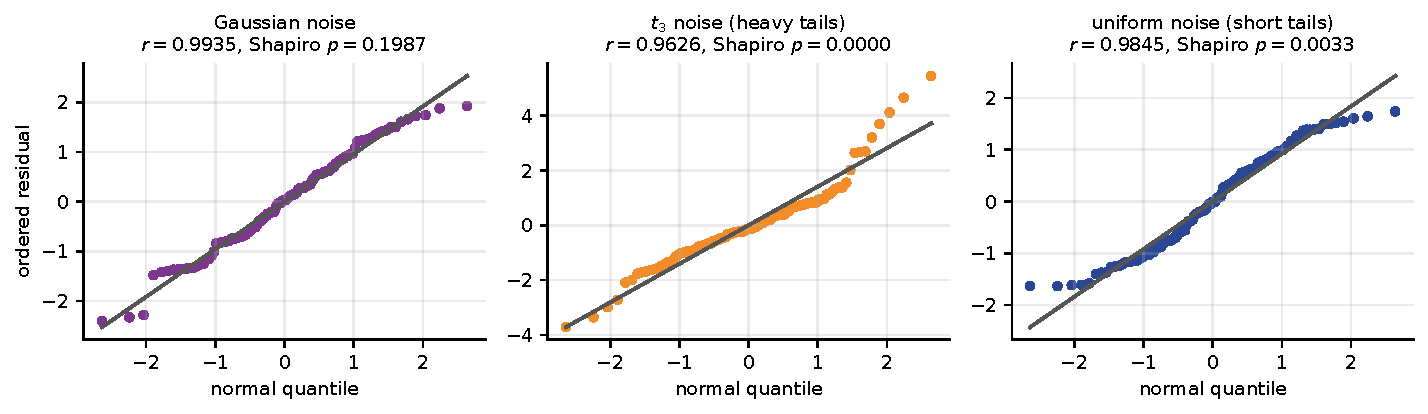
\includegraphics[width=0.80\textwidth]{qqplots.pdf}
\caption{Three sets of $120$ residuals. Gaussian sits on the line. $t_3$ bends
\emph{away} at both ends --- heavy tails. Uniform bends \emph{towards} the
line --- short tails. All three correlations exceed $0.97$, which is why the
picture beats the summary statistic here.}
\label{fig:qq}
\end{figure}

Read the shape, not the number. All three correlations are above $0.97$, and
yet only one of the three sets is Normal. Heavy tails show as an S-curve that
falls below the line on the left and rises above it on the right; short tails
show the mirror image. Neither is fatal for the coefficients, and both
invalidate the $p$-values.

\subsection{A checklist you can run in five lines}

\begin{tryit}
For any fitted regression, produce these four plots and look at them before
you report anything:
\begin{enumerate}[leftmargin=*]
  \item residuals against fitted values --- linearity and constant variance;
  \item a normal Q--Q plot of the residuals --- normality;
  \item residuals against observation order or time --- independence;
  \item leverage $h_i = 1/n + (x_i-\bar x)^2/S_{xx}$ against the residual ---
    influential points. Flag any $h_i > 2p/n$.
\end{enumerate}
On the four Anscombe datasets these four plots give four different verdicts
from the identical $R^2 = 0.666$. That is the point of the exercise.
\end{tryit}

% =========================================================================
\section{Over-fitting and its detection}
\label{sec:overfit}

\subsection{What over-fitting is}

A model \textbf{over-fits} when it has started to learn the noise in the
training rows --- structure that is real in those rows and will not repeat.
The signature is two error curves that separate: training error keeps falling,
error on unseen rows stops falling and turns upward.

Why it must happen for polynomials is arithmetic. A degree-$d$ polynomial has
$d+1$ free coefficients. Given $n$ points with distinct $x$, a polynomial of
degree $n-1$ passes exactly through every one of them, noise included, and
$R^2 = 1$ on the training set. Perfect training fit is a symptom, not an
achievement.

The running example is $25$ points drawn from $y = \sin(2\pi x) + \varepsilon$
with $\sigma = 0.25$ on $[0,1]$. Because the truth and the noise level are
known, the experiment can be graded: no model can do better than an RMSE of
$0.25$ on fresh data.

\begin{figure}[htbp]
\centering
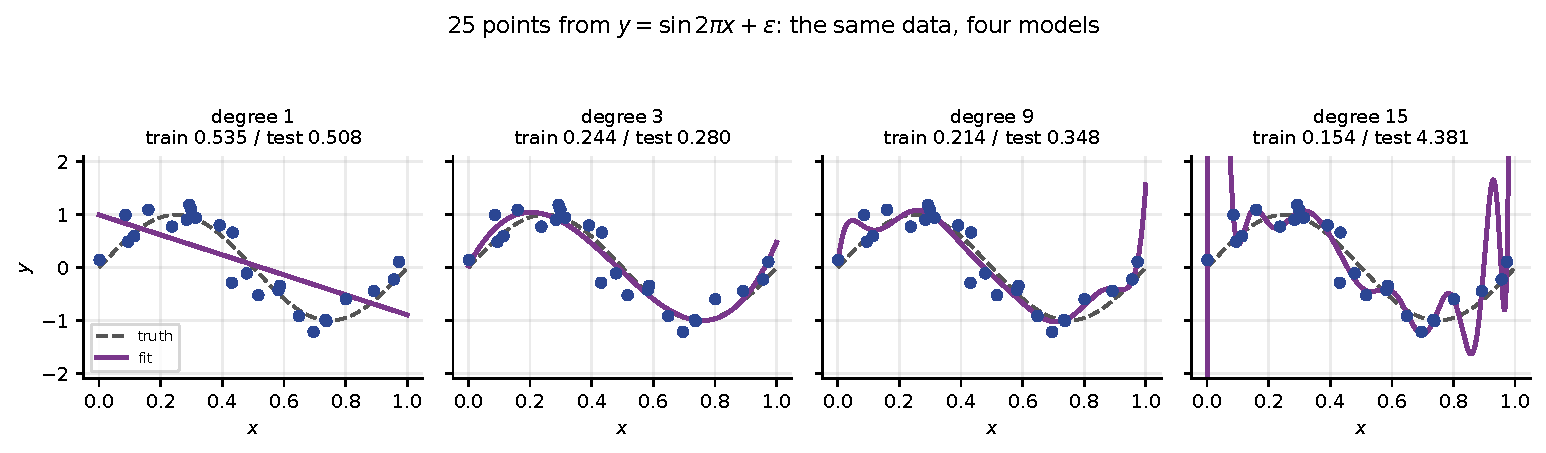
\includegraphics[width=0.80\textwidth]{polyfits.pdf}
\caption{The same $25$ points, four models. Degree $1$ cannot bend
(\emph{under-fitting}); degree $3$ tracks the truth; degree $9$ ripples;
degree $15$ passes near every point and leaves the dashed truth entirely.}
\label{fig:polyfits}
\end{figure}

\subsection{The degree curve}
\label{sec:degcurve}

\begin{lstlisting}
rng = np.random.default_rng(3)             # DATA seed: fixes these 25 points
x_train = np.sort(rng.uniform(0, 1, 25))
y_train = np.sin(2*np.pi*x_train) + rng.normal(0, 0.25, 25)
x_test  = np.sort(rng.uniform(0, 1, 2000))
y_test  = np.sin(2*np.pi*x_test) + rng.normal(0, 0.25, 2000)
for d in range(21):
    c = np.polynomial.Polynomial.fit(x_train, y_train, d)
    tr = np.sqrt(np.mean((y_train - c(x_train))**2))
    te = np.sqrt(np.mean((y_test  - c(x_test ))**2))   # 2000 fresh rows
\end{lstlisting}
\begin{codeout}
degree  params  train RMSE   test RMSE
   0       1      0.7507        0.7523
   1       2      0.5347        0.5084
   2       3      0.5290        0.5147
   3       4      0.2441        0.2795   <-- test minimum
   4       5      0.2433        0.2820
   5       6      0.2273        0.2828
   8       9      0.2255        0.2842
   9      10      0.2143        0.3484
  12      13      0.1843        0.5966
  13      14      0.1617        1.4545
  15      16      0.1540        4.3811
  18      19      0.1518       36.7111
  19      20      0.1473      533.7692
  20      21      0.1466      153.1554
train RMSE strictly non-increasing? True   largest increase -3.29e-05
test minimum at degree 3, RMSE 0.2795   (noise floor 0.2500)
degree 20: train RMSE 0.1466 (60.1% of degree-3), test RMSE 153.1554 (547.9x worse)
\end{codeout}

Three readings.

\textbf{The training curve is monotone, and this was checked, not assumed.}
Every one of the twenty steps reduced the training RMSE, from $0.7507$ to
$0.1466$; the largest single change was $-3.29\times10^{-5}$, i.e.\ negative.
This is the same theorem as Section~\ref{sec:noisecols}: a degree-$(d{+}1)$
model contains every degree-$d$ model.

\textbf{The test curve turns at degree 3.} Its minimum, $0.2795$, is a
whisker above the noise floor of $0.2500$, which is the best any model could
do. After that it rises, slowly at first and then not slowly: $0.35$ at degree
$9$, $4.38$ at degree $15$, $153$ at degree $20$.

\textbf{Between degree 3 and degree 20, the training score improved by
$\mathbf{40\%}$ and the model became unusable} --- $548$ times worse on fresh
data. If your only instrument is the training score, that entire journey looks
like progress.

\begin{figure}[htbp]
\centering
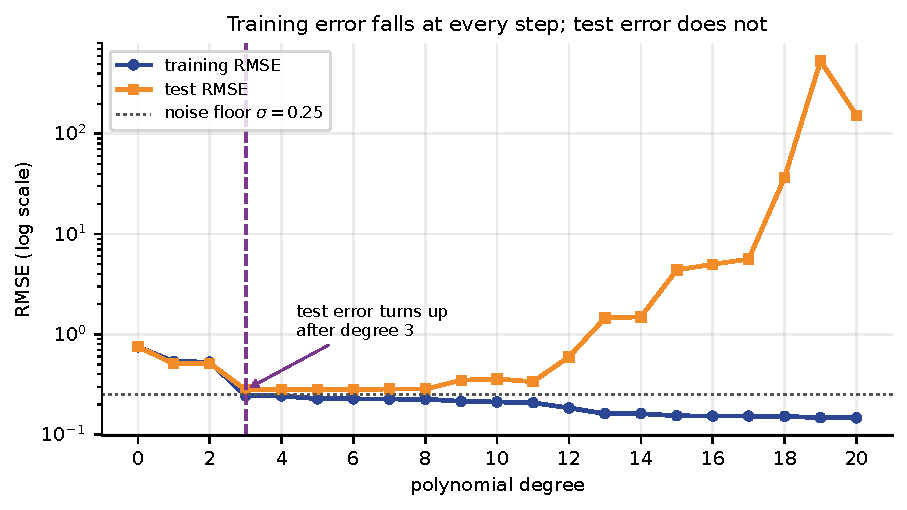
\includegraphics[width=0.56\textwidth]{overfit.pdf}
\caption{Log scale on the vertical axis, or the right-hand end would not fit
on the page. The blue curve is monotone by construction; the orange curve owes
you nothing, and after degree $3$ it stops paying.}
\label{fig:overfit}
\end{figure}

\begin{caution}[Read the tail of the table honestly]
Degree $19$ has a larger test RMSE ($533.8$) than degree $20$ ($153.2$). The
curve is not monotone once the design matrix is badly conditioned: past that
point the numbers are dominated by numerical behaviour and by which particular
$25$ rows we drew. The teaching content is the \emph{turn at degree 3}, not the
ordering of the last few entries.
\end{caution}

\subsection{Over-fitting depends on $n$, not just on the model}
\label{sec:nmatters}

Change only the number of training rows and rerun.

\begin{codeout}
 n_train   best degree   test RMSE at best   test RMSE at degree 20
     15         3              0.2959               13292.3268
     25         5              0.3102                2867.4761
     50         6              0.2634                   0.3256
    200         5              0.2547                   0.2656
   1000         7              0.2536                   0.2572
\end{codeout}

At $n = 15$, degree $20$ produces a test RMSE of thirteen thousand. At
$n = 1000$, the \emph{same} twenty-one-parameter model gives $0.2572$ against
a best of $0.2536$ and a noise floor of $0.2500$ --- it costs $0.0036$, about
one and a half per cent.

\begin{keyidea}
Over-fitting is not a property of the model. It is a property of the model
\emph{and} the amount of data. ``How complex a model may I use?'' has no answer
until you say $n$.
\end{keyidea}

\subsection{It happens on real data too}
\label{sec:realoverfit}

\begin{lstlisting}
Xtr, Xte, ytr, yte = train_test_split(Xd, yd, test_size=0.25, random_state=0)
for deg in (1, 2, 3):
    pipe = make_pipeline(PolynomialFeatures(deg, include_bias=False),
                         LinearRegression()).fit(Xtr, ytr)
    print(pipe.score(Xtr, ytr), cross_val_score(pipe, Xtr, ytr, cv=5).mean(),
          pipe.score(Xte, yte))
\end{lstlisting}
\begin{codeout}
model                          train R2    5-fold CV R2   held-out R2   params
linear (10 features)         +0.5554        +0.5224        +0.3594          10
degree-2 polynomial          +0.6469        +0.3827        +0.2440          65
degree-3 polynomial          +0.9179     -1212.1828       -22.0428         285
predicting the training mean for every patient: held-out R2 -0.0001
\end{codeout}

$285$ parameters against $331$ training rows. The training column goes
\emph{up} at every row of the table and the held-out column goes \emph{down} at
every row. Reading only the training column, you would ship the worst of the
three models. And the last line supplies the yardstick: predicting a constant
scores $-0.0001$ on the held-out rows, so the degree-3 model at $-22.04$ is
more than twenty times worse than doing nothing at all.

% =========================================================================
\section{Cross-validation as the detector}
\label{sec:cv}

\subsection{The idea}

The over-fitting section detected the turn using a test set. That is not a
method you can use during model development, because a test set that has been
consulted repeatedly is no longer a test set --- every choice you make from it
leaks information about it into your model.

\textbf{$k$-fold cross-validation}, introduced with the splitting strategies of
Unit~IV, solves this using only the training rows. Split them into $k$ roughly
equal parts (folds). For each fold in turn, fit
the model on the other $k-1$ folds and score it on the held-out fold. Average
the $k$ scores.

Every row is used for testing exactly once and for training $k-1$ times. You
obtain a held-out estimate without spending a held-out set, and because you get
$k$ scores rather than one, you also get a spread. The cost is $k$ model fits.
The extreme case $k = n$ is \textbf{leave-one-out cross-validation} (LOOCV):
$n$ fits, each on $n-1$ rows, and no randomness at all, because there is only
one way to leave one row out.

\begin{caution}[The test set is not part of this]
The test set is opened once, at the end, to report a number --- never to choose
a degree, a scaler or a threshold. Cross-validation happens entirely inside the
training rows. If you have used the test set to make a decision, whatever you
report from it is a training score wearing a disguise.
\end{caution}

\subsection{Cross-validation finds the turn}
\label{sec:cvdetect}

\begin{lstlisting}
from sklearn.model_selection import KFold, cross_val_score
from sklearn.pipeline import make_pipeline
from sklearn.preprocessing import PolynomialFeatures

kf = KFold(5, shuffle=True, random_state=0)
for d in range(16):
    pipe = make_pipeline(PolynomialFeatures(d), LinearRegression())
    cv = -cross_val_score(pipe, x_train[:, None], y_train, cv=kf,
                          scoring="neg_root_mean_squared_error").mean()
\end{lstlisting}
\begin{codeout}
degree   train RMSE   5-fold CV RMSE   LOOCV RMSE     test RMSE
   0      0.7507          0.7769        0.7819        0.7523
   1      0.5347          0.6319        0.5895        0.5084
   2      0.5290          0.9097        0.6396        0.5147
   3      0.2441          0.3239        0.2799        0.2795
   4      0.2433          0.6234        0.3163        0.2820
   5      0.2273          0.6711        0.2912        0.2828
   6      0.2273          1.3741        0.4295        0.2823
   7      0.2257          4.6874        0.5433        0.2843
   8      0.2255          3.1131        1.3879        0.2842
   9      0.2143         32.7952        0.4516        0.3484
  10      0.2114        143.9583        2.8380        0.3592
  11      0.2076        710.1122       17.7364        0.3367
  12      0.1843        661.0253       23.7564        0.5966
  13      0.1617       1959.3824       13.9714        1.4545
  14      0.1616       7218.1668       73.5354        1.4941
  15      0.1540      23379.8414       49.8944        4.3811
train RMSE picks degree 15 (the largest offered)
5-fold CV  picks degree 3
LOOCV      picks degree 3
the test set says       3
\end{codeout}

The training column picks the largest model on offer, as it always will. Both
cross-validated columns pick degree $3$ --- the same answer the test set gives
--- \textbf{using nothing but the $25$ training rows}. That single table is the
argument for cross-validation.

\begin{figure}[htbp]
\centering
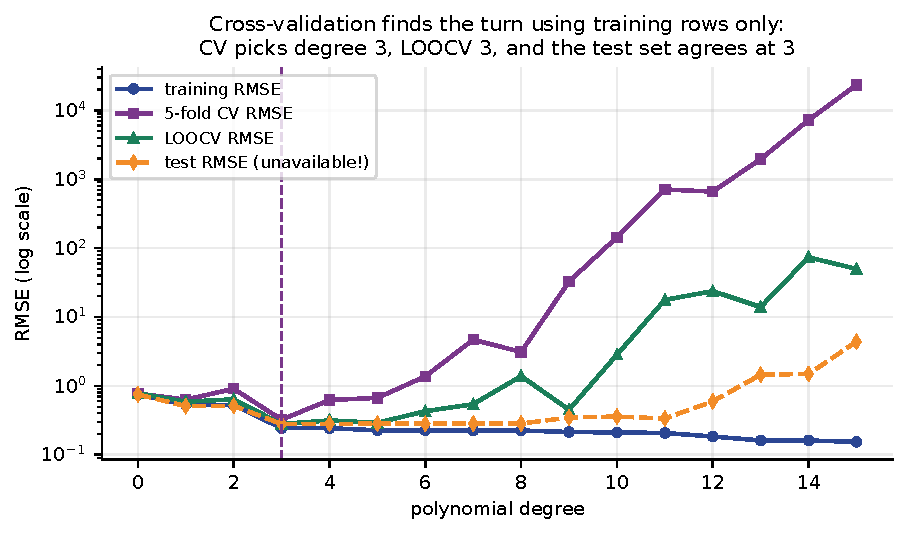
\includegraphics[width=0.56\textwidth]{cvdetect.pdf}
\caption{Four curves. The orange dashed one is the test error, drawn here only
because this is a demonstration; in a real project you may not look at it. The
purple and green curves reproduce its minimum without it.}
\label{fig:cvdetect}
\end{figure}

Note that the CV columns are much larger than the test column at high degree.
That is expected and it is not a defect: each CV fit uses only $20$ of the
$25$ rows, so its polynomial is even less constrained than the one fitted to
all $25$. Cross-validation is a slightly \emph{pessimistic} estimate of the
error of the final model, and pessimism in this direction is exactly what you
want from a detector.

\subsection{Why not just one validation split?}
\label{sec:lottery}

The obvious cheaper alternative is to hold out one chunk of the training rows
and use it to choose. It works, on average, and the variance is the problem.

\begin{lstlisting}
for seed in range(10):
    xa, xb, ya, yb = train_test_split(x_train, y_train, test_size=0.4,
                                      random_state=seed)
    curve = [rmse(yb, Polynomial.fit(xa, ya, d)(xb)) for d in range(11)]
    print(int(np.argmin(curve)))
\end{lstlisting}
\begin{codeout}
ten different single validation splits of the same 25 rows
  degree chosen by each split: [3, 3, 3, 3, 4, 5, 3, 3, 3, 3]
  chosen degrees range from 3 to 5
  spread of the estimated RMSE at degree 3: 0.2243 to 0.4415
5-fold CV RMSE at degree 3 (one number, no split lottery): 0.3239
\end{codeout}

Seven of the ten splits chose degree $3$ and three did not. Worse, the
\emph{estimate} of the error at degree $3$ ranged from $0.2243$ to $0.4415$ ---
a factor of two --- from nothing but which rows happened to land in which half.
Report the first and you look good; report the second and you look bad; neither
is a property of the model.

\begin{figure}[htbp]
\centering
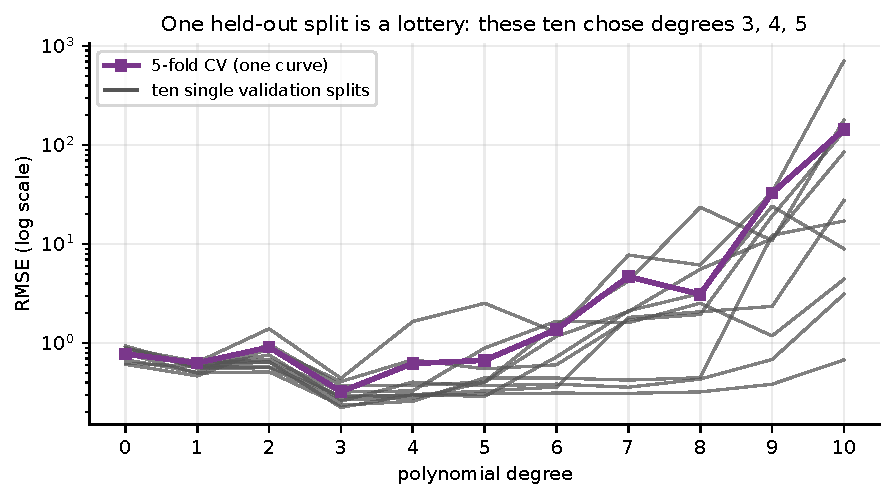
\includegraphics[width=0.56\textwidth]{valsplit.pdf}
\caption{Ten single validation splits of the same $25$ rows in grey, and the
5-fold CV curve in purple. $k$-fold averages the lottery away and uses every
row for training.}
\label{fig:valsplit}
\end{figure}

\subsection{Choosing $k$}

\begin{center}
\begin{tabular}{@{}lp{4.6cm}p{5.0cm}@{}}
\toprule
& \textbf{Bias of the estimate} & \textbf{Variance and cost}\\
\midrule
$k = 2$ & pessimistic: each fit sees only half the data &
  cheap, two fits, but noisy\\[4pt]
$k = 5$ or $10$ & small; the usual default &
  moderate: five or ten fits\\[4pt]
$k = n$ (LOOCV) & almost none: each fit sees $n-1$ rows &
  $n$ fits, and the training sets overlap almost completely, so the $n$
  scores are highly correlated\\
\bottomrule
\end{tabular}
\end{center}

In the table of Section~\ref{sec:cvdetect}, LOOCV tracked the test curve more
closely at small degree --- $0.2799$ against a test $0.2795$ at degree $3$ ---
because each of its fits saw $24$ rows rather than $20$. It cost $25$ fits
against $5$. On $25$ rows that is free; on $250{,}000$ rows it is not.

\begin{keyidea}[The rule that outranks the choice of $k$]
\textbf{Everything the model learns must be refitted inside every fold.} A
polynomial degree, a scaler, a feature selection, a decision threshold. If a
choice was made using all the rows and then cross-validated, the resulting
score is not a held-out score. \texttt{Pipeline} exists precisely so that
doing this correctly is easier than doing it wrongly, which is why every
listing in this section wraps its preprocessing in one.
\end{keyidea}

\begin{tryit}
Re-run the degree sweep with \texttt{KFold(5, shuffle=True, random\_state=1)}
instead of \texttt{random\_state=0}. The individual CV numbers will move ---
they are averages over a random partition --- but the chosen degree should stay
at $3$. If it moves, that tells you the choice between two adjacent degrees is
not supported by $25$ rows, which is itself worth knowing.
\end{tryit}

% =========================================================================
\section{Summary}

\begin{enumerate}[leftmargin=*]
  \item ``Closest'' is a choice. On the five points the direct slope is
    $0.6000$, the inverse slope $1.0000$ and the orthogonal slope $0.7208$;
    each minimises its own criterion and nothing else, and
    $b^{\mathrm{dir}}/b^{\mathrm{inv}} = r^2 = 0.6$.
  \item \textbf{Assume $\varepsilon_i \sim \mathcal{N}(0,\sigma^2)$
    independently, write the likelihood, take logarithms, and
    $\ell = \text{const} - \mathrm{SSE}/(2\sigma^2)$. Maximising $\ell$ is
    identical to minimising the SSE.} Least squares is the Gaussian maximum
    likelihood estimator.
  \item $\sigma^2$ is a positive multiplier of $-\mathrm{SSE}$ and cannot move
    the estimate: the same $b_1 = 0.60000$ maximised the likelihood at
    $\sigma^2 = 0.48$ and at $\sigma^2 = 1$.
  \item $\hat\sigma^2_{\mathrm{ML}} = \mathrm{SSE}/n$ is \textbf{biased
    downwards} by the factor $(n-2)/n$. Over $20{,}000$ datasets with
    $\sigma^2 = 4$ and $n = 10$ it averaged $3.2117$ against a predicted
    $3.2000$, and was too small in $73.4\%$ of runs. Use
    $s^2 = \mathrm{SSE}/(n-2)$.
  \item Change the noise to Laplace and the MLE becomes least \emph{absolute}
    deviations, which recovered the true intercept to $0.23$ against least
    squares' $1.09$ on contaminated data.
  \item $R^2 = 1 - \mathrm{SS_{res}}/\mathrm{SS_{tot}} = 1 - 2.40/6.00 =
    0.6000$ on the five points, equal to $r^2$ and to
    $b_1^2 S_{xx}/S_{yy}$, and $s = 0.8944$.
  \item \textbf{$R^2$ never falls when you add a predictor.} Twenty-seven
    pure-noise columns on $30$ rows took it from $0.2413$ to $0.9401$, and the
    smallest of the $27$ steps was $+3\times10^{-6}$.
  \item Adjusted $R^2$ caught that ($-0.7375$), but on $442$ rows with $410$
    junk columns it read $+0.6597$ while cross-validation read $-5.7605$. It
    is a penalty, not a test.
  \item Held-out $R^2$ has \textbf{no lower bound}: $-3$ on three numbers by
    hand, $-1.106$ for a degree-14 fit, $-22.04$ for a degree-3 polynomial on
    diabetes against $-0.0001$ for predicting the mean.
  \item Anscombe's four datasets share every summary statistic and
    $R^2 = 0.666$. The residual diagnostics separate them completely:
    curvature $R^2 = 1.0000$ for II, largest residual $2.80\times$ the next for
    III, leverage $1.0000$ and an undefined deleted slope for IV.
  \item Heteroscedastic data gave $R^2 = 0.9267$ with a residual sd ratio of
    $1.82$ and Breusch--Pagan $p \approx 2\times10^{-6}$. Coefficients survive
    it; every standard error and $p$-value does not. $\log y$ took the
    statistic from $22.91$ to $3.24$ ($p = 0.072$) --- most of the way, not all
    of it.
  \item Over-fitting: training RMSE fell at all $20$ steps while test RMSE
    turned up after \textbf{degree 3}, reaching $153$ at degree $20$ ---
    $548\times$ worse. At $n = 1000$ the same degree $20$ costs $0.0036$ in
    RMSE, $1.4\%$.
  \item \textbf{5-fold CV and LOOCV both chose degree 3, the same answer as
    the test set, using only the training rows}, while the training score
    chose the largest model offered. A single validation split chose $3$, $4$
    or $5$ depending on the seed, and estimated the degree-3 error anywhere
    between $0.2243$ and $0.4415$.
\end{enumerate}

% =========================================================================
\section{Practice questions}
\label{sec:questions}

Attempt these before reading Section~\ref{sec:solutions}. Questions
\ref{q:three}, \ref{q:derive}, \ref{q:sigma}, \ref{q:r2hand}, \ref{q:adj} and
\ref{q:neg} are pure hand work and are the ones most likely to appear on a
paper.

\begin{enumerate}[leftmargin=*]
  \item\label{q:three} Four points: $(1,1)$, $(2,3)$, $(3,2)$, $(4,4)$.
    (a) Compute $\bar x$, $\bar y$, $S_{xx}$, $S_{yy}$ and $S_{xy}$.
    (b) Give the direct regression slope, the inverse regression slope
    expressed as $y$ against $x$, and the orthogonal slope. (c) Verify that
    the ratio of the first two is $r^2$. (d) Which line would you use to
    predict $y$ from $x$, and why?

  \item\label{q:derive} Starting from a blank page, derive the maximum
    likelihood estimator of $(\beta_0, \beta_1)$ for simple linear regression.
    State the model and its assumptions, write the likelihood, take
    logarithms, and show \emph{explicitly} why the answer does not depend on
    $\sigma^2$. Then state what changes if the noise is Laplace rather than
    Gaussian.

  \item\label{q:sigma} A regression on $n = 6$ points gives
    $\mathrm{SSE} = 12$. (a) Give $\hat\sigma^2_{\mathrm{ML}}$ and the
    unbiased $s^2$. (b) If the true $\sigma^2$ is $3$, what is
    $\mathbb{E}[\hat\sigma^2_{\mathrm{ML}}]$, and by what percentage does the
    MLE understate the truth on average? (c) At what $n$ does that
    understatement fall below $1\%$?

  \item\label{q:r2hand} Data: $x = (0,1,2,3,4)$, $y = (1,3,2,5,4)$.
    (a) Fit the direct regression line by hand. (b) Tabulate the fitted values
    and residuals and compute $\mathrm{SS_{tot}}$, $\mathrm{SS_{res}}$ and
    $\mathrm{SS_{reg}}$. (c) Give $R^2$ and check it two other ways.
    (d) Give $s$, the standard error of the estimate.

  \item\label{q:adj} A model with $n = 20$ and one predictor has $R^2 = 0.60$.
    You add eight more predictors and $R^2$ rises to $0.68$.
    (a) Compute adjusted $R^2$ for both models. (b) Which model does adjusted
    $R^2$ prefer? (c) Holding $R^2$ fixed at $0.68$, at what $p$ does adjusted
    $R^2$ first become negative? (d) Explain in one sentence why $R^2$ rose,
    without assuming the new predictors are useful.

  \item\label{q:neg} On three held-out points $y = (4, 6, 8)$ your model
    predicts $(10, 6, 2)$. (a) Compute $R^2$. (b) What constant prediction
    would give $R^2 = 0$, and what would the constant $5$ give? (c) Explain in
    two sentences why $R^2$ is bounded below by $0$ on training data and not on
    held-out data.

  \item\label{q:debug} A colleague reports: ``I fitted a degree-3 polynomial
    expansion of the ten diabetes features and got $R^2 = 0.918$. This is much
    better than the plain linear model's $0.555$, so we should use it.''
    Their notebook, in order: (i) load; (ii) build the degree-3 features;
    (iii) fit on all $331$ training rows; (iv) print
    \texttt{model.score(X\_train, y\_train)}. Identify every problem, quantify
    the damage using measured numbers from these notes, and write the
    corrected four lines of code.

  \item\label{q:resid} You fit a model and get $R^2 = 0.89$. The residuals
    against fitted values form a clear wedge, narrow on the left and wide on
    the right. (a) Name the violated assumption. (b) State precisely what is
    and is not invalidated. (c) Give a test statistic you could compute and
    how. (d) Give one remedy and the measured effect it had in
    Section~\ref{sec:hetero}.

  \item\label{q:overfit} From the degree table of Section~\ref{sec:degcurve}:
    (a) Which degree does each of ``lowest training RMSE'', ``lowest 5-fold CV
    RMSE'' and ``lowest test RMSE'' select? (b) Prove that training RMSE cannot
    increase with degree. (c) By what percentage does training RMSE improve
    from degree $3$ to degree $20$, and by what factor does test RMSE worsen?
    (d) Explain the apparent contradiction in one sentence.

  \item\label{q:design} You are given $60$ rows and one predictor, and asked
    to choose a polynomial degree between $1$ and $10$ and then report an
    honest estimate of how well the final model will do on new data. Write the
    protocol as a numbered list. For each step say what data it may use, and
    cite one measured number from these notes justifying the step.
\end{enumerate}

% =========================================================================
\section{Solutions}
\label{sec:solutions}

\textbf{\ref{q:three}.} (a) Both means are $2.5$. The $x$-deviations are
$-1.5$, $-0.5$, $0.5$, $1.5$ and the $y$-deviations $-1.5$, $0.5$, $-0.5$,
$1.5$, so
$S_{xx} = 2.25 + 0.25 + 0.25 + 2.25 = 5$, likewise $S_{yy} = 5$, and
$S_{xy} = 2.25 - 0.25 - 0.25 + 2.25 = 4$.

(b) Direct $= S_{xy}/S_{xx} = 4/5 = 0.8$. Inverse, as $y$ against $x$,
$= S_{yy}/S_{xy} = 5/4 = 1.25$. For the orthogonal slope the covariance matrix
is $\tfrac{1}{3}\bigl(\begin{smallmatrix}5&4\\4&5\end{smallmatrix}\bigr)$,
which has equal diagonal entries, so its eigenvectors are
$(1,1)/\sqrt2$ and $(1,-1)/\sqrt2$ and the leading slope is exactly $1$.

(c) $0.8/1.25 = 0.64$, and
$r^2 = S_{xy}^2/(S_{xx}S_{yy}) = 16/25 = 0.64$. \checkmark

(d) The direct line, because the task named is predicting $y$ from $x$. Note
that all three slopes are different and $0.8 < 1.0 < 1.25$.

\medskip
\textbf{\ref{q:derive}.} \emph{Model.}
$y_i = \beta_0 + \beta_1 x_i + \varepsilon_i$ with
$\varepsilon_i \sim \mathcal{N}(0,\sigma^2)$, independent, $i = 1,\dots,n$;
the $x_i$ are fixed and known. Assumptions: linear conditional mean, constant
variance, independence, normality.

\emph{Likelihood.} With $e_i = y_i - \beta_0 - \beta_1x_i$,
\[
  L = \prod_{i=1}^n (2\pi\sigma^2)^{-1/2}
      \exp\!\left(-\frac{e_i^2}{2\sigma^2}\right)
    = (2\pi\sigma^2)^{-n/2}\exp\!\left(-\frac{1}{2\sigma^2}\sum_i e_i^2\right).
\]

\emph{Log-likelihood.}
$\ell = -\tfrac{n}{2}\log(2\pi) - \tfrac{n}{2}\log\sigma^2
        - \tfrac{1}{2\sigma^2}\sum_i e_i^2$.

\emph{Why $\sigma^2$ drops out.} Only the third term contains $\beta_0$ and
$\beta_1$. Write $\ell = A - cS(\beta_0,\beta_1)$ where
$A = -\tfrac n2\log(2\pi) - \tfrac n2\log\sigma^2$ is free of the
$\beta$'s and $c = 1/(2\sigma^2) > 0$. Maximising $A - cS$ over
$(\beta_0,\beta_1)$ is minimising $S$, and the value of $c$ changes the
\emph{height} of the objective but not its \emph{argmax}, because $c$ is a
strictly positive constant. Hence the ML estimates are the least squares
estimates for every $\sigma^2 > 0$. Setting $\partial S/\partial\beta_0 =
\partial S/\partial\beta_1 = 0$ gives the normal equations and
$\hat\beta_1 = S_{xy}/S_{xx}$, $\hat\beta_0 = \bar y - \hat\beta_1\bar x$.

\emph{Laplace noise.} The density is $\tfrac{1}{2b}e^{-|e|/b}$, so
$\ell = -n\log(2b) - \tfrac1b\sum_i|e_i|$ and the MLE minimises
$\sum_i|e_i|$: least absolute deviations. Measured in
Section~\ref{sec:laplace}, the LAD fit recovered the true intercept $2.00$ as
$2.77$ where least squares gave $3.00$; the two slopes were indistinguishable
on that single sample, which is itself worth noting.

\medskip
\textbf{\ref{q:sigma}.} (a) $\hat\sigma^2_{\mathrm{ML}} = 12/6 = 2.0$ and
$s^2 = 12/4 = 3.0$.
(b) $\mathbb{E}[\hat\sigma^2_{\mathrm{ML}}] = \tfrac{n-2}{n}\sigma^2
= \tfrac46 \times 3 = 2.0$; the understatement is $2/n = 33.33\%$.
(c) $2/n < 0.01$ requires $n > 200$, so $n \ge 201$.

\begin{codeout}
SSE 12.0  n 6
sigma^2 MLE      = 12.0/6 = 2.0000
sigma^2 unbiased = 12.0/4 = 3.0000
E[MLE] = (n-2)/n * sigma^2 = 0.6667 * 3.0 = 2.0000
understated by 33.33%
\end{codeout}

Note that here the unbiased estimate happens to equal the true $\sigma^2$
exactly; that is a coincidence of the chosen $\mathrm{SSE}$, not a property.

\medskip
\textbf{\ref{q:r2hand}.} (a) $\bar x = 2$, $\bar y = 3$. The $x$-deviations are
$-2,-1,0,1,2$ and the $y$-deviations $-2,0,-1,2,1$, so $S_{xx} = 10$,
$S_{yy} = 10$ and $S_{xy} = 4+0+0+2+2 = 8$. Hence $b_1 = 8/10 = 0.8$ and
$b_0 = 3 - 0.8\times2 = 1.4$.

(b) Fitted $(1.4, 2.2, 3.0, 3.8, 4.6)$; residuals $(-0.4, 0.8, -1.0, 1.2,
-0.6)$. $\mathrm{SS_{tot}} = 10$, $\mathrm{SS_{res}} = 0.16 + 0.64 + 1.00 +
1.44 + 0.36 = 3.60$, $\mathrm{SS_{reg}} = 6.40$.

(c) $R^2 = 1 - 3.6/10 = 0.64$. Check one: $\mathrm{SS_{reg}}/\mathrm{SS_{tot}}
= 6.4/10 = 0.64$, and independently $b_1^2S_{xx} = 0.64 \times 10 = 6.40$.
Check two: $r^2 = 8^2/(10 \times 10) = 0.64$.

(d) $s = \sqrt{3.6/(5-2)} = \sqrt{1.2} = 1.0954$.

\begin{codeout}
xbar 2.0 ybar 3.0  Sxx 10.0 Syy 10.0 Sxy 8.0
b1 0.8000  b0 1.4000
fitted    [1.4 2.2 3.  3.8 4.6]
residuals [-0.4  0.8 -1.   1.2 -0.6]
SSres 3.6000  SStot 10.0000  SSreg 6.4000  b1^2*Sxx 6.4000
R2 0.6400   r^2 0.6400   s 1.0954
\end{codeout}

\medskip
\textbf{\ref{q:adj}.} (a) $p = 1$:
$1 - 0.40 \times \tfrac{19}{18} = 1 - 0.4222 = 0.5778$. $p = 9$:
$1 - 0.32 \times \tfrac{19}{10} = 1 - 0.608 = 0.3920$.

(b) The first, clearly: adjusted $R^2$ fell by $0.19$ even though $R^2$ rose
by $0.08$. Eight predictors bought $0.08$ of $R^2$, and eight degrees of
freedom cost far more than that.

(c) Solve $1 - 0.32\times\tfrac{19}{19-p} < 0$, i.e.\ $6.08 > 19-p$, i.e.\
$p > 12.92$. So $p = 13$ is the first negative value, at $-0.0133$.

(d) Because $R^2$ cannot fall when a predictor is added: the previous fit
remains available with the new coefficient set to zero, so the minimised
$\mathrm{SS_{res}}$ can only decrease. A rise in $R^2$ is therefore evidence of
nothing.

\begin{codeout}
n=20 p=1  R2 0.6000  adjusted 0.5778
n=20 p=9  R2 0.6800  adjusted 0.3920
   n=20 p=12 R2 0.6800  adjusted +0.1314
   n=20 p=13 R2 0.6800  adjusted -0.0133
   n=20 p=14 R2 0.6800  adjusted -0.2160
\end{codeout}

\medskip
\textbf{\ref{q:neg}.} (a) $\bar y_{\mathrm{test}} = 6$;
$\mathrm{SS_{tot}} = 4 + 0 + 4 = 8$;
$\mathrm{SS_{res}} = 36 + 0 + 36 = 72$; $R^2 = 1 - 72/8 = -8$.

(b) The constant $6$ --- the test mean --- gives exactly $0$. The constant $5$
gives $\mathrm{SS_{res}} = 1 + 1 + 9 = 11$ and $R^2 = 1 - 11/8 = -0.375$: even
the wrong constant beats the model.

(c) On training data the intercept is fitted, so $\hat y = \bar y$ is one of
the candidate fits and least squares cannot do worse than it; therefore
$\mathrm{SS_{res}} \le \mathrm{SS_{tot}}$ and $R^2 \ge 0$. On held-out data
$\bar y_{\mathrm{test}}$ was never available to the fitting procedure, so
nothing constrains $\mathrm{SS_{res}}$ relative to $\mathrm{SS_{tot}}$ and
$R^2$ is unbounded below.

\begin{codeout}
SStot 8.0  SSres 72.0  R2 -8.0000
R2 of the constant 6.0  0.0000
R2 of the constant 5.0  -0.3750
\end{codeout}

\medskip
\textbf{\ref{q:debug}.} Three problems, of increasing seriousness.

\emph{One --- the number reported is a training score.}
\texttt{model.score(X\_train, y\_train)} is $R^2$ on the rows the model was
fitted to. It is not an estimate of anything about future data.

\emph{Two --- the comparison is between models of different sizes, using a
metric that cannot make that comparison.} Degree-3 expansion of ten features
gives $285$ predictors against the linear model's $10$. $R^2$ cannot decrease
when predictors are added (Section~\ref{sec:noisecols}), so
$0.918 > 0.555$ was guaranteed before anyone looked at the data. The measured
demonstration: $27$ columns of \emph{pure noise} raised $R^2$ from $0.2413$ to
$0.9401$ on $30$ rows.

\emph{Three --- and this is the one that matters --- the model is
catastrophically over-fitted.} $285$ parameters on $331$ rows. From
Section~\ref{sec:realoverfit}: 5-fold CV $R^2 = -1212.18$ and held-out
$R^2 = -22.04$, against $-0.0001$ for predicting the training mean. The
proposal is to replace a model scoring $+0.36$ on held-out data with one
scoring $-22$.

A fourth point worth making: adjusted $R^2$ would not have saved them. On
diabetes with $410$ junk columns it read $+0.6597$ while cross-validation read
$-5.7605$ (Section~\ref{sec:adjr2}).

\emph{Corrected code.}
\begin{lstlisting}
pipe = make_pipeline(PolynomialFeatures(deg, include_bias=False),
                     LinearRegression())
print(cross_val_score(pipe, X_train, y_train,
                      cv=KFold(5, shuffle=True, random_state=0),
                      scoring="r2").mean())          # choose deg by THIS
pipe.fit(X_train, y_train)
print(pipe.score(X_test, y_test))                    # report once, at the end
\end{lstlisting}
\begin{codeout}
model                          train R2    5-fold CV R2   held-out R2   params
linear (10 features)         +0.5554        +0.5224        +0.3594          10
degree-2 polynomial          +0.6469        +0.3827        +0.2440          65
degree-3 polynomial          +0.9179     -1212.1828       -22.0428         285
\end{codeout}

\medskip
\textbf{\ref{q:resid}.} (a) Constant variance --- homoscedasticity. The data is
heteroscedastic, with $\sigma$ growing with $\hat y$.

(b) The coefficient estimates remain \emph{unbiased}: least squares needs no
constant-variance assumption for that, and by Gauss--Markov it is only the
efficiency that is lost. What is invalidated is everything computed from a
single $\sigma$: the standard errors of the coefficients, every $t$ and $F$
statistic, every $p$-value, and both confidence and prediction intervals. A
prediction interval will be too wide at small $\hat y$ and far too narrow at
large $\hat y$, which is the dangerous direction.

(c) The Breusch--Pagan test: regress the squared residuals on the fitted
values, take $nR^2$ from that auxiliary regression, and compare it to a
$\chi^2$ with one degree of freedom. In Section~\ref{sec:hetero} this gave
$22.9065$ with $p \approx 2\times10^{-6}$.

(d) Transform the response. Taking $\log y$ moved the Breusch--Pagan statistic
from $22.9065$ to $3.2426$ ($p = 0.0717$) and the ratio of upper-half to
lower-half residual sd from $1.82$ to $0.89$. Note that $p = 0.072$ is not a
clean pass: the transform removed most of the trend in the variance but not
all of it. Weighted least squares is the alternative when a transform is not
acceptable, or not enough.

\medskip
\textbf{\ref{q:overfit}.} (a) Lowest training RMSE: \textbf{degree 20} (or
$15$ if the sweep stops there) --- always the largest offered. Lowest 5-fold CV
RMSE: \textbf{degree 3}. Lowest test RMSE: \textbf{degree 3}.

(b) The set of degree-$d$ polynomials is a subset of the set of
degree-$(d{+}1)$ polynomials --- take the degree-$(d{+}1)$ coefficient to be
zero. Least squares returns the minimum of the training SSE over the set it is
given, and the minimum over a superset cannot exceed the minimum over a subset.
Hence training SSE, and therefore training RMSE, is non-increasing in $d$. This
was verified: the largest single-step change over $20$ steps was
$-3.29\times10^{-5}$.

(c) Training RMSE fell from $0.2441$ to $0.1466$, an improvement of
$\mathbf{39.9\%}$. Test RMSE rose from $0.2795$ to $153.1554$, worse by a
factor of $\mathbf{547.9}$.

(d) There is no contradiction: the extra flexibility was spent fitting the
particular noise realisation in those $25$ rows, which is real structure in the
training data and pure interference in any other data.

\medskip
\textbf{\ref{q:design}.} A defensible protocol.

\begin{enumerate}[leftmargin=*]
  \item \textbf{Split first.} Hold out, say, $15$ of the $60$ rows as a test
    set and put them away. \emph{May use:} nothing but a random number
    generator. \emph{Why:} any decision made with these rows makes the final
    number a training score. In Section~\ref{sec:cvdetect} the training score
    chose the largest model on offer.
  \item \textbf{Cross-validate inside the remaining 45.} For each degree
    $1..10$, run 5-fold CV and record the mean RMSE. \emph{May use:} the $45$
    training rows only. \emph{Why:} CV chose degree $3$ --- the same answer as
    the test set --- using nothing but training rows.
  \item \textbf{Do not use a single validation split.} \emph{Why:} ten
    different $60/40$ splits of the same $25$ rows chose degrees $3$, $4$ and
    $5$, and estimated the degree-3 error anywhere between $0.2243$ and
    $0.4415$ (Section~\ref{sec:lottery}).
  \item \textbf{Wrap every fitted step in a \texttt{Pipeline}} so that the
    polynomial expansion and any scaling are refitted inside each fold.
    \emph{Why:} anything the model learns from all $45$ rows before the folds
    are cut is no longer held out.
  \item \textbf{Prefer the simpler model on a tie.} If two degrees are within
    one CV standard error, take the smaller. \emph{Why:} at $n = 15$ degree
    $20$ produced a test RMSE of $53{,}293$; complexity is cheap to add and
    expensive when wrong (Section~\ref{sec:nmatters}).
  \item \textbf{Refit the chosen degree on all $45$ rows}, then score once on
    the $15$ test rows and report that number. \emph{Why:} it is the only
    number in the whole procedure computed on data no decision used.
  \item \textbf{Report the residual plot with it.} \emph{Why:} four datasets
    with $R^2 = 0.666$ had four different problems (Section~\ref{sec:resplot}).
  \item \textbf{Say $n$ when you report the degree.} \emph{Why:} the same
    degree-$20$ model was catastrophic at $n = 15$ and cost $0.0036$ at
    $n = 1000$.
\end{enumerate}

% =========================================================================
\section{References and further reading}

All links were checked on 22 August 2026. Free resources are marked
\textbf{[free]}.

\subsection*{Textbooks}

\begin{itemize}[leftmargin=*]
  \item Bishop, \emph{Pattern Recognition and Machine Learning}, Springer,
    2006. \textbf{The prescribed text for this lecture.} \S1.2.5 ``Curve
    fitting re-visited'' --- the maximum likelihood derivation of
    Section~\ref{sec:central}, done for polynomial regression; \S3.1.1
    ``Maximum likelihood and least squares'', the same argument in matrix form
    with the precision parameter $\beta = 1/\sigma^2$; \S1.1 and \S1.3 for the
    over-fitting figures and model selection; \S3.2 the bias--variance
    decomposition.
  \item James, Witten, Hastie, Tibshirani and Taylor, \emph{An Introduction to
    Statistical Learning with Python}. \textbf{[free]} \S3.1.3 ``Assessing the
    accuracy of the model'' --- $\mathrm{RSE}$, $R^2$, and the identity
    $R^2 = r^2$ for simple regression; \S3.3.3 ``Potential problems'', which is
    Section~\ref{sec:adequacy} of these notes in six numbered headings;
    \S5.1 the validation set approach, LOOCV and $k$-fold cross-validation, and
    \S5.1.4 on the bias--variance trade-off for $k$.
    \url{https://www.statlearning.com/}
  \item M\"uller and Guido, \emph{Introduction to Machine Learning with
    Python}, O'Reilly, 2016. \S5.1 cross-validation --- \S5.1.1 in
    scikit-learn, \S5.1.2 the benefits, \S5.1.3 stratified and other
    splitters; \S2.3.3 on linear models and the training/test gap. Notebooks
    \textbf{[free]}:
    \url{https://github.com/amueller/introduction_to_ml_with_python}
  \item Deisenroth, Faisal and Ong, \emph{Mathematics for Machine Learning}.
    \textbf{[free]} Ch.~9, ``Linear Regression'': \S9.2 parameter estimation,
    which does maximum likelihood \emph{first} and least squares as its
    consequence --- the order used in these notes; \S9.2.2 on overfitting in
    linear regression.
    \url{https://mml-book.github.io/}
  \item Murphy, \emph{Probabilistic Machine Learning: An Introduction}.
    \textbf{[free]} \S11.2 ``Least squares linear regression'', including
    \S11.2.3 on the MLE for $\sigma^2$ and why it is biased, and \S11.4 on
    robust linear regression --- the Laplace likelihood of
    Section~\ref{sec:laplace}, worked out properly.
    \url{https://probml.github.io/pml-book/book1.html}
  \item Hastie, Tibshirani and Friedman, \emph{The Elements of Statistical
    Learning}, 2e, Springer. \textbf{[free]} \S7.2 bias, variance and model
    complexity --- the theory behind Figure~\ref{fig:overfit}; \S7.10
    cross-validation, including the choice of $k$ and the one-standard-error
    rule.
    \url{https://hastie.su.domains/ElemStatLearn/}
\end{itemize}

\subsection*{Online courses}

\begin{sloppypar}
\begin{itemize}[leftmargin=*]
  \item \textbf{NPTEL, Linear Regression Analysis and Forecasting} --- Prof.\
    Shalabh, IIT Kanpur. The closest match anywhere to the vocabulary this
    examination uses: the direct, inverse and orthogonal regression methods of
    Section~\ref{sec:direct} are named and derived exactly as they are here,
    and the maximum likelihood estimation of the simple linear model is a
    lecture of its own. \textbf{[free]}
    \url{https://nptel.ac.in/courses/111104098}
  \item \textbf{NPTEL, Introduction to Machine Learning} --- Prof.\ Balaraman
    Ravindran, IIT Madras; the reference course for the semester. The linear
    regression week covers least squares and the bias--variance trade-off.
    \textbf{[free]} \url{https://nptel.ac.in/courses/106106139}
  \item \textbf{SWAYAM} --- the national portal hosting NPTEL, with the
    enrolment and certification route. \textbf{[free]}
    \url{https://swayam.gov.in/}
  \item \textbf{Google Machine Learning Crash Course} --- the ``Linear
    regression'', ``Overfitting'' and ``Datasets, generalization'' modules;
    short, browser-based, and a good first pass before the mathematics.
    \textbf{[free]}
    \url{https://developers.google.com/machine-learning/crash-course}
\end{itemize}
\end{sloppypar}

\subsection*{Videos}

\begin{itemize}[leftmargin=*]
  \item StatQuest with Josh Starmer, \emph{Maximum Likelihood, clearly
    explained!!!} --- the likelihood-versus-probability distinction of
    Section~\ref{sec:mle} at a whiteboard, in six minutes. Watch this first if
    the word ``likelihood'' has not yet clicked. \textbf{[free]}
    \url{https://youtu.be/XepXtl9YKwc}
  \item StatQuest with Josh Starmer, \emph{R-squared, Clearly Explained!!!} ---
    $\mathrm{SS_{tot}}$, $\mathrm{SS_{res}}$ and the ratio, drawn rather than
    derived. Covers the ``$R^2$ always goes up'' point of
    Section~\ref{sec:noisecols}. \textbf{[free]}
    \url{https://youtu.be/2AQKmw14mHM}
  \item StatQuest with Josh Starmer, \emph{Machine Learning Fundamentals:
    Cross Validation} --- $k$-fold and leave-one-out in five minutes, with the
    ``do not touch the test set'' rule stated plainly. \textbf{[free]}
    \url{https://youtu.be/fSytzGwwBVw}
  \item StatQuest with Josh Starmer, \emph{Machine Learning Fundamentals: Bias
    and Variance} --- the theory underneath Figure~\ref{fig:overfit}: why the
    test curve has to turn. \textbf{[free]}
    \url{https://youtu.be/EuBBz3bI-aA}
  \item CampusX, \emph{Regression Metrics $\vert$ MSE, MAE \& RMSE $\vert$ R2
    Score \& Adjusted R2 Score} --- the whole of Section~\ref{sec:r2} in
    examination vocabulary, including the adjusted $R^2$ formula and when it
    goes negative. \textbf{[free]}
    \url{https://youtu.be/Ti7c-Hz7GSM}
  \item Mahesh Huddar, \emph{Linear Regression Numerical Example with one
    Independent Variable} --- a full hand calculation of the kind in
    Section~\ref{sec:r2hand}, at the speed a written paper requires.
    \textbf{[free]} \url{https://youtu.be/OXMATSKUlRY}
\end{itemize}

\subsection*{Documentation and interactive explainers}

\begin{itemize}[leftmargin=*]
  \item Seeing Theory (Brown University), \emph{Chapter 6: Regression
    Analysis} --- drag the points of \textbf{Anscombe's quartet} and watch the
    least-squares line and the $\mathrm{SSE}$ move. The best five minutes you
    can spend on Section~\ref{sec:anscombe}. \textbf{[free]}
    \url{https://seeing-theory.brown.edu/regression-analysis/index.html}
  \item MLU-Explain, \emph{Linear Regression} --- Jared Wilber's scrollable
    explainer covering least squares, $R^2$ and the closed form, with every
    figure interactive. \textbf{[free]}
    \url{https://mlu-explain.github.io/linear-regression/}
  \item scikit-learn user guide: \emph{Metrics and scoring} (\S3.4, with the
    exact definition of \texttt{r2\_score} and the note that it can be
    negative); \emph{Cross-validation: evaluating estimator performance}
    (\S3.1, with \texttt{KFold}, \texttt{LeaveOneOut} and the
    \texttt{Pipeline} warning). \textbf{[free]}
    \url{https://scikit-learn.org/stable/modules/model_evaluation.html} \\
    \url{https://scikit-learn.org/stable/modules/cross_validation.html}
  \item scikit-learn example, \emph{Underfitting vs.\ Overfitting} --- the
    figure of Section~\ref{sec:degcurve} as a runnable script, using the same
    cosine target and polynomial degrees. \textbf{[free]}
    \url{https://scikit-learn.org/stable/auto_examples/model_selection/plot_underfitting_overfitting.html}
\end{itemize}

\subsection*{Articles}

\begin{itemize}[leftmargin=*]
  \item F.\ J.\ Anscombe, ``Graphs in Statistical Analysis'', \emph{The
    American Statistician} \textbf{27}(1), 1973, pp.\ 17--21. The four
    datasets of Section~\ref{sec:anscombe}, and the sentence they exist to
    support: \emph{``make both calculations and graphs. Both sorts of output
    should be studied; each will contribute to understanding.''}
  \item Matejka and Fitzmaurice, ``Same Stats, Different Graphs'', ACM CHI
    2017 --- how to \emph{generate} Anscombe-like datasets, including the
    Datasaurus. Convincing proof that summary statistics do not determine a
    dataset. \textbf{[free]}
    \url{https://www.research.autodesk.com/publications/same-stats-different-graphs/}
\end{itemize}

\enlargethispage{4\baselineskip}
\notesources{\AMLUnitVSources}

\end{document}
